
\chapter{Introduction}
Modern communication systems often incorporate numerous, uncoordinated users competing for a limited resource. In this work, a game theoretic approach considers a wireless communication network with uncoordinated macrocell users and femtocell base stations. The goal of this approach is to find Nash equilibrium (NE) in which femtocell base stations optimize individual utility while ensuring interference tolerances are not violated for macrocell users. 
Previous work has shown solutions for systems in which femtocell base stations transmit over a single input, single output (SISO) channel; therefore the multiple input, multiple ouput (MIMO) case is investigated here. 
\par
In the communications context, distributed optimization is often preferable in order to minimize the overhead of information passing required by central optimization. 
This work focuses on achieving NE using distributed solutions. 


\section{Notation}
The following notation is used throughout the remainder. 
$E\{\cdot\}$ is the expectation operator.
Vectors are denoted by bold font, lower-case letters ($\mathbf{x}$) and are assumed to be column vectors.
Matrices are denoted by bold font, upper-case letters ($\mathbf{X}$). The transpose and hermetian of $\mathbf{X}$ are denoted by $\mathbf{X}^T$ and $\mathbf{X}^H$ respectively.
$\mathbf{I}$ denotes the identity matrix. $\mathrm{diag}(\mathbf{x})$ denotes the diagonal matrix created by placeing the elements of the vector $\mathbf{x}$ along the diagonal. $\mathrm{trace}(\cdot)$ is the trace operator. The operator $(\cdot)^+$ yields the argument if greater than 0, and 0 otherwise.


\section{Relevant Tools/Theory}\label{tools}
It is useful to first review relevant game theoretic tools. Together, these tools provide a series of steps to follow in order to determine Nash Equilibrium via distributed solutions. 
\par
We consider a game in which $F$ players each choose a strategy $\mathbf{b}_{f}$ from a set of possible strategies $\mathcal{B}_f$. The vector $\mathbf{b}=[\mathbf{b}_{1}^T, \mathbf{b}_2^T... \mathbf{b}_{f}^T]^T \in \mathcal{B}$ represents the strategies of all players. Each player has a utility function $U_f(\mathbf{b})$ which it attempts to maximize through the choice of $\mathbf{b}_{f}$. The set of strategies available to a player, $\mathbf{b}_{f} \in\mathcal{B}_f$, may be dependent on the strategies of other players $\mathbf{b}_{j}, j \neq f $.

\begin{enumerate}
\item The potential function: a central optimization problem used to identify Nash equilibrium of a game.
\begin{itemize}
\item
\textbf{Definition:}  A potential function is any function
$ \Psi(\mathbf{b})$ which satisfies:
\begin{equation}\label{potential_game_condition}
\frac{\partial \Psi(\mathbf{b})}{\partial \mathbf{b}_{f}}
 =
 \frac{\partial U_f(\mathbf{b})}{\partial \mathbf{b}_{f}}.
\end{equation} 

In words, $ \Psi(\mathbf{b})$ is a function whose gradient with respect to the strategy $\mathbf{b}_{f}$ of a player, is equal to the gradient of that player's utility function with respect to $\mathbf{b}_{f}$.

\item \textbf{Result:} Global optima of a potential function are Nash Equilibria \cite{monderer1996potential}.
\item \textbf{Note:} Not all games admit a potential function.


\end{itemize}

\item Normalized Nash equilibrium: if we consider the case in which the set $\mathcal{B}$ is convex and $U_f(\mathbf{b})$ is concave, non-decreasing and has continuous first derivative in $\mathbf{b}_{f}$, the resulting optimal strategy for each player (and thus any Nash equilibrium) will satisfy the necessary and sufficient KKT conditions. A normalized Nash equilibrium (NNE) is a Nash equilibrium for which the dual variables of all players are equal up to a constant. 
Intuitively, this can be thought of as a Nash equilibrium for which each players is "charged" an equal amount (up to a constant) for any change in strategy.

\item The Concave N-Person game: A framework for proving existence and uniqueness of normalized Nash equilibrium.

\begin{itemize}
\item
\textbf{Definition:} A game in which all $U_f(\mathbf{b})$ are concave with respect to $\mathbf{b}_f$ and the set of possible $\textbf{b}\in\mathcal{B}$ is convex. 
\item 
\textbf{Existence of Nash Equilibrium:} Pure Strategy NEs exist for Concave N-Person games \cite[Thm1]{rosen1964existence}. 
\item
\textbf{Uniqueness of Nash Equilibrium:} In general, multiple NNEs may exist for a game. However, sufficient conditions for uniqueness are shown in \cite[Thm4]{rosen1964existence} and introduced in the following. 
Taking the gradient of each $U_f(\mathbf{b})$ with respect to the chosen strategy $\textbf{b}_f$ we first form the vector
\begin{equation}
g(\mathbf{b})= 
\begin{bmatrix}
\nabla U_{1}(\mathbf{b})
\\
\nabla U_{2}(\mathbf{b})
\\
\vdots\\
\nabla U_{F}(\mathbf{b})
\end{bmatrix}.
\end{equation}
We define the Jacobian of $g(\mathbf{b}) $ as the matrix valued function $G(\mathbf{b}) $.
Negative definiteness of the matrix $[G(\mathbf{b})+G^{T}(\mathbf{b})] $ is a sufficient condition for uniqueness of a NNE.
\item \textbf{Result 1:} For a Concave N-Person game admitting a potential function, the potential function is concave, allowing for use of convex optimization tools to find a NE. 

\end{itemize}




\item Distributed Optimization: Solving a central optimization problem using multiple processes in parallel.
In particular, the dual ascent method described in \cite{boyd2011distributed} is used in this work.

\textbf{Distributed Dual Ascent} 
\begin{itemize}
\item For a central optimization problem (obtained using a potential function in this work), determine the dual problem to the central, primal problem.
\item Evaluate if the dual problem can be separated into sub-problems, each with independent optimization variables.
\item Perform an ascent of the dual problem by iterating the following:
\begin{enumerate}
\item Solve the separate dual function of the sub-problems.
\item Broadcast these solutions and perform the gradient step of the dual problem.
\end{enumerate}
\end{itemize}

If the problem is convex with strong duality, the dual ascent will converge to the optimal (in this case a Nash Equilibrium).

\end{enumerate}




\section{Outline}
The above tools are used in the steps outlined below. 
\begin{itemize}
\item 
\ref{genmodel}: Introduce the system model for the general game.
\item 
\ref{genproblem}: Analyze the general setup to see why further refinements are useful in arriving at a distributed solution. 
\item
\ref{conmodel}: Introduce refinements to the system model.
\item 
\ref{conproblem}: Develop a distributed solution using the refined system model.
\item 
\ref{numerical}: Discuss numerical results of the proposed solution. 
\end{itemize}
\chapter{System Model}

\section{General System Model}\label{genmodel}

\subsection{Players: Femtocell Base Stations}


Each player of the game, a femtocell base station (FBS) $f \in \{1 ... F\}$ , is characterized by the following.
\begin{itemize}
\item 
$T_{f}$ antennas to transmit to $K_{f}$ femtocell users (we assumed that $T_{f} \geq K_{f}$). Each femtocell user $i = [1... \;K_{f}]$ has a signal to interference plus noise ratio (SINR) $\gamma_{f,i}$. The vector of user SINRs for FBS $f$ is $\boldsymbol{\gamma}_{f} = [\gamma_{f,1}...\; \gamma_{,K_{f}}]$
\\
\item 
	A beamforming matrix $\mathbf{U}_{f} \in \mathbb{C}_{T_{f} \times K_{f}}$ such that the transmitted 		
	signal is $\mathbf{s}_{f
	}= \mathbf{U}_{f}\mathbf{x}_{f}$. The 		
	vector of symbols for users of FBS $f$, $\mathbf{x}_{f}$, is  normalized such that $E\{\|x_{f,i}
	\|_2^2\}=1$ and $E\{\mathbf{x}_{f}\mathbf{x}_{f}^H\}=\mathbf{I}_{K_{f} \times K_{f}}$.
\\
\item 
	An average power constraint $E\{trace(\mathbf{U}_{f}^H\mathbf{U}_{f})\} \leq P^{Total}_{f} $.

\item 
	A cost function $U_{f}(\boldsymbol{\gamma}_{f}) =
	\sum_{i=1}^{K_{f}}
    	 U_{f,i}(\gamma_{f,i}) $
    	in which $U_{f,i}(\cdot)$ is a non-decreasing function describing the utility obtained by each user, $i$, of FBS $f$.

\item 
	Perfect knowledge of the downlink channel to the users of FBS $f$ given by the matrix $\mathbf{H}_f \in \mathbb{C}_{K_{f} \times T_{f}} $ .
% TODO(Simulate degradation with incomplete CSI solution?)
\\
\item
	 FBSs are assumed to be spaced far apart in distance such that they cause no interference to one another.
\end{itemize}

\subsection{Macrocell Users}
Macrocell users $m \in \{1 ... M\}$ introduce constraints into the game. These users are characterized by the following.

\begin{itemize}
\item 
	Received interference constraint
	$E\{\sum^F_{f=1} \tilde{\mathbf{h}}_{m,f}^T  \mathbf{U}_{f}					
	\mathbf{U}_{f}^{H} \tilde{\mathbf{h}}_{m,f}^*\} \leq I^{Threshold}		
	_{m} $. In which $\tilde{\mathbf{h}}_{m,f}$ is the channel from FBS $f$ to macro user $m$.

\item 
	FBS $f$ is assumed to know the downlink channel matrix $\tilde{\mathbf{H}}_{f} \in \mathbb{C}_{M \times T_{f}}$ to all $M$ macrocell users.
\\
\end{itemize}

\subsection{Femtocell Users}
\begin{itemize}

\item User $i$ of FBS $f$ has signal to interference plus noise ratio (SINR)
	\begin{equation*}
	\gamma_{f,i} = \frac{\|\mathbf{h}^H_{f,i}\mathbf{u}_{f,i}\|^2}
	{\sigma^2_{\text{noise}}   +
	\underbrace{
	 \sum_{\tilde{f}=1, \tilde{f}\neq f}^{f} \sum_{u=1}^{K_{\tilde{f}}}
	\|\mathbf{h}^H_{\tilde{f},u}\mathbf{u}_{\tilde{f},i}\|^2}_{\mathrm{inter-cell}}
	 + 
	 \underbrace{
	 \sum_{\tilde{k}=1, \tilde{k}\neq i}^{K_f}
	 \|\mathbf{h}^H_{f,\tilde{k}}\mathbf{u}_{f,\tilde{k}}\|^2}_{\mathrm{intra-cell}}},
	  \; i \in \{1 ... K_f\}
	  \end{equation*}
\\
with noise power $\sigma^2_{\text{noise}}.$
\\

By the FBS spacing assumption above, this reduces to
	\begin{equation*}
	\gamma_{f,i} = \frac{\|\mathbf{h}^H_{f,i}\mathbf{u}_{f,i}\|^2}
	{\sigma^2_{\text{noise}} 
	 + \sum_{\tilde{k}=1, \tilde{k}\neq i}^{K_f}
	  \|\mathbf{h}^H_{f,\tilde{k}}\mathbf{u}_{f,\tilde{k}}\|^2},
	  \; i \in \{1 ... K_f\}
	\end{equation*}

\end{itemize}





\subsection{General Optimization Problem}\label{genproblem}

Each FBS $f$ attempts to maximize utility function $U_{f}(\cdot)$ while satisfying the interference constraints imposed by the macrocell users and a transmission power constraint. This results in the following optimization problem at each FBS.
\par

	\begin{subequations}
	\label{optim}
	\begin{align}
	    \underset{\mathbf{U}_{f} }{\text{minimize  }} \;
	    & - \sum_{i=1}^{K_f}
    	U_{f,i}(\gamma_{f,i}) \label{player_opt} \\
	    \text{subject to  } \; &
	   \sum^F_{f=1} \tilde{\mathbf{h}}_{m,f}^H  \mathbf{U}_{f}^*		
	\mathbf{U}_{f}^{T} \tilde{\mathbf{h}}_{m,f} \leq I^{Threshold}		
	_{m} & m \in \{1 ...M\} 
		\label{interference_const_gen}\\
        & trace(\mathbf{U}_{f}^H\mathbf{U}_{f}) \leq P^{Total}_{f} \label{power_const_gen}\\
        & \mathbf{h}_{f,i}^H\mathbf{u}_{f,i} =0\ & \; \forall \; j \in \{1... K_{f}\}\backslash i,\; \forall \; i\in \{1 ... K_{f}\} \label{zf_const_gen}
	\end{align}
	\end{subequations}


The constraints in \eqref{zf_const_gen} imply that $\mathbf{U}_{f}$ is chosen such that  
	\begin{equation}\label{zf_snr}
	\gamma_{f,i} = \frac{\|\mathbf{h}^H_{f,i}\mathbf{u}_{f,i}\|^2}
	{\sigma^2_{noise}  
	}
	= 
	\frac{\mathbf{u}^H_{f,i}\mathbf{h}_{f,i}\mathbf{h}^H_{f,i}\mathbf{u}_{f,i}}
	{\sigma^2_{noise}  
	},
	\end{equation}
	which is a convex function with respect to $\mathbf{u}_{f,i}$.
%	As a result, $U_{f,i}(\gamma_{f,i}) $ is concave with respect to $\gamma_{f,i}$.
	
\subsection{Concave N-Person game analysis of general setup}
In this section, the convexity of the resulting problem is analyzed to investigate if the system satisfies the conditions of the concave N-person game described \ref{tools}. 

\begin{enumerate}
\item
First, we check that constraints \eqref{interference_const_gen}-\eqref{zf_const_gen} form a convex, closed and bounded set. 

\begin{itemize}

\item
	Constaint \eqref{interference_const_gen} contains $M$ quadratic constraints on $\mathbf{U}_f$, each of which 
	can be rewritten  as

\begin{gather*}
	\sum_{f=1}^{f}
	trace(\mathbf{U}_{f}^H \tilde{\mathbf{h}}_{m,f} \tilde{\mathbf{h}}_{m,f}^H \mathbf{U}_f )\leq 
	I^{Threshold}_{m}.
\end{gather*}
This can be further decomposed into a sum of independent, quadratic form terms
	\begin{gather*}
	\sum_{f=1}^{f}
	\sum_{i=1}^{f_i}
	\mathbf{u}_{f,i}^H\tilde{\mathbf{h}}_{m,f} \tilde{\mathbf{h}}_{m,f}^H
	\mathbf{u}_{f,i} \leq I^{Threshold}_{m}
	\end{gather*}
in which each matrix $\tilde{\mathbf{h}}_{m,f} \tilde{\mathbf{h}}_{m,f}^H$ is positive semi-definite \cite[p.~8,9]{BoV:04}. The union of independent convex sets forms a convex set \cite{BoV:04}, therefore this constraint is convex. 
%This is essentially high dimensional ellipsoid.

\item \
	Constraint \eqref{power_const_gen} can be similarly decomposed into the sum
	\begin{gather*}
		\sum_{i=1}^{K_{f}}\mathbf{u}_{f,i}^{H} \mathbf{I} 		
		\mathbf{u}_{f,i} \leq  P^{Total}_{f}
	\end{gather*}
	in which $\mathbf{I}$ is positive definite, creating a strictly convex set.

\item 
	Constaint \eqref{zf_const_gen} is an affine constraint. 
		\begin{gather*}
		\mathbf{h}_{f,j}^T \mathbf{u}_{f,i} =0
		\end{gather*}
%Note that affine constaints to not have to satisfy Slater's condition
\end{itemize}


\item Second, we check if the utility function is concave.
\begin{itemize}
\item 
Let us consider the SINR at femto-user i of FBS f given by
	\begin{equation*}\label{zf_snr}
	\gamma_{f,i} = 
	\frac{\mathbf{u}^H_{f,i}\mathbf{h}_{f,i}\mathbf{h}^H_{f,i}\mathbf{u}_{f,i}}
	{\sigma^2_{noise}  
	}.
	\end{equation*}
	Since
	 $\mathbf{h}_{f,i}\mathbf{h}^H_{f,i}$ is positive semi-definite, $\gamma_{f,i}$ is convex in ${\mathbf{u}_{f,i}}$. 
	 The resulting composition $U_{f,i}(\gamma_{f,i}) $ is concave only if $U_{f,i}(\cdot) $ is concave and non-increasing; violating the non-decreasing definition of $U_{f,i}(\cdot) $.
If $U_{f,i}(\cdot) $ is a general, non-decreasing function, the result is quasiconvex \cite[p.~102]{BoV:04}. If $U_{f,i}(\cdot) $ is  non-decreasing and convex, the resulting
   function is convex which can be solved using concave programming to find a \emph{maximum}.
\end{itemize}

\end{enumerate}

\subsection{Potential Game for the General Problem}
Under the current system model, the game is not a concave N-person game. Nevertheless, since the utility function of individual FBSs are independent of the strategy chosen by other FBSs, due to the spacing assumption, the game still admits a potential function. The investigation of distributed concave programming techniques for solving this general formulation of the problem is left for future work. 

\section{Concave System Model}\label{conmodel}

The general setup of the game proposed in the previous section does not enable the use of the N-person concave game framework to find normalized Nash equilibrium. We propose a more restrictive model characterized by a unique, normalized Nash equilibrium. This NNE can be be found via a single convex optimization problem which may be solved in a distributed manner across FBSs and macro-users in the network.
\par
Rather than jointly optimizing the power allocation and the zero-forcing beamformers, we now pre-select normalized, zero-forcing beamformers independently, \emph{before} the allocation of powers.
As we will see later, one result of this restriction is that the degrees of freedom available at the FBS cannot be fully exploited during power allocation. 

\subsection{Players: Femtocell Base Stations}\label{conmodel_fbs}
Femtocell base stations are adapted from the general setup to the restricted setup by the following.
\begin{itemize}
\item 
	FBSs with multiple antennas ($T_f \geq 1$) can beamform their transmission using the precoding 	
	matrix $\mathbf{U}_{f} \in \mathbb{C}_{T_{f} \times K_{f}}$ .
	The columns of $\mathbf{U}_{f}$ are now \emph{normalized} such that 
	 $\|\mathbf{u}_{f,i}\|^2 =1 \;\forall i \in \{1 ... K_{f}\}$.
\\

\item 
$\mathbf{U}_f$ is selected as a pseudo-inverse to $\mathbf{H}_f$.
Such that
\begin{gather*}
\mathbf{H}_{f}  \mathbf{U}_{f} = \mathbf{I}.
\end{gather*} 


\item  
	FBS $f$ allocates the transmit powers using the diagonal, power allocation  	
	matrix $\mathrm{diag}(\mathbf{p}_{f})$ with $p_{f,i} \geq 0, \forall i \in \{1 ... K_{f}\}$
such that the transmitted 		
	signal is 
	$\mathbf{s}_{f	}= \mathbf{U}_{f} 
	\mathrm{diag}(\mathbf{p}_{f})^{\frac{1}{2}}
	\mathbf{x}_{f}$. We define the vector variable $\mathbf{p}^T= [\mathbf{p}_1^T, \mathbf{p}_2^T...\mathbf{p}_{f}^T]$ containing the transmit power vectors of all FBSs.
\\
\item 
	FBS $f$ enforces the power constraint given by
	\begin{gather*}
	\text{trace}(E[\mathbf{s}_f\mathbf{s}_f^H]) =
	\sum_{i=1}^{K_{f}} p_{f,i}
	  \leq P^{Total}_{f}.
	  	\end{gather*}


% TODO(Simulate degradation with incomplete CSI solution?)


\item 
	Utility function of FBS f is given by $U_{f}(\boldsymbol{\gamma}_f) =
	\sum_{i=1}^{K_{f}}
    	U_{f,i}(\gamma_{f,i}) $
    	where all $U_{f,i}(\cdot)$ are non-decreasing and
    	\emph{strictly} concave.
\item The SINR of the femto-user $i$ in FBS $f$ is given by
\begin{equation}\label{zf_snr}
	\gamma_{f,i} =\frac{\sum_{i=i}^{K_{f}}
 p_{f,i}\|h_{f,i}u_{f,i}\|^2}
	{\sigma^2_{noise}  
	}.
	\end{equation}

\end{itemize}

\subsection{Macrocell Users}
No change with respect to the general setup.

\subsection{Femtocell Users}\label{conmodel_fuser}
No change with respect to the general setup.



\subsection{Optimization Problem of Player $f$}\label{conproblem}
The optimization problem at FBS $f$ for the system described in \ref{conmodel_fbs}-\ref{conmodel_fuser} is given by

	\begin{subequations}
	\label{optim}
	\begin{align}
	    \underset{\mathbf{p}_{f} }{\text{minimize  }} \;
	    & - \sum_{i=1}^{K_f}
    	U_{f,i}(\gamma_{f,i}) \label{player_opt_c} \\
	    \text{subject to  } \; &
	  \sum^F_{f=1} E\{ \tilde{\mathbf{h}}_{m,f}^T  \mathbf{s}_{f} 						
	\mathbf{s}_{f}^{H} \tilde{\mathbf{h}}_{m,f}^* \}
	=
	\sum_{f=1}^{f}	\sum_{i=1}^{K_f}
	 p_{f,i}\|\tilde{\mathbf{h}}_{m,f}^T \mathbf{u}_{f,i}\|^2_2
	\leq I^{Threshold}		
	_{m} & m \in \{1 ...m\} 
		\label{interference_const_c}\\
        & 
        	\sum_{i=1}^{K_{f}} p_{f,i}
	   \leq P_{f}^{\text{Total}}  \label{power_const_c}\\
        & p_{f,i} \geq 0 &  i\in \{1 ...K_{f}\} \label{pos_power_const_c}
	\end{align}
	\end{subequations}

Note that because $\mathbf{U}_{f}$ is pre-selected as a pseudo-inverse to  $\mathbf{H}_f$, the zero-forcing constraint \eqref{zf_const_gen} has been removed.

\subsection{Concave N-Person game analysis of concave setup}
The convexity of the resulting problem is analyzed to investigate if this system admits the concave N-person game framework. 

\begin{enumerate}


\item
First, check that the constraints form a convex, closed and bounded set. 

\begin{itemize}

\item
	Note that \eqref{interference_const_c} includes $m$ affine constraints in $\mathbf{p}_{f}$.

\begin{gather*}
	  \sum^F_{f=1} \tilde{\mathbf{h}}_{m,f}^T  \mathbf{s}_{f} 						
	\mathbf{s_{f}^{H}} \tilde{\mathbf{h}_{m,f}^*} 
	=
	\sum_{f=1}^{f}	\sum_{i=1}^{K_f}
	p_{f,i}\|\tilde{\mathbf{h}}_{m,f}^T \mathbf{u}_{f,i}\|
	\leq I^{Threshold}_{m} 
\end{gather*}

\item \
	Constraint \eqref{power_const_c} is  affine in $\mathbf{p}_{f}$.
	
\item \
	Constraint \eqref{pos_power_const_c} is affine in $\mathbf{p}_{f}$.
\end{itemize}

%Note that affine constaints to not have to satisfy Slater's condition

\item The utility function was defined to be concave in $p_{f,i}$. 

\end{enumerate}

This problem satisfies the conditions for the concave N-person game and therefore a  normalized Nash equilibrium exists due to 
\cite[Thm1]{rosen1964existence}.

Assuming continuously differentiable $U_{f,i}(\gamma_{f,i})$ and $\gamma_{f,i}(p_{f,i})$, the diagonal elements of $[G(b,r)+G^{T}(b,r)] $ correspond to
\begin{equation}
\underbrace{U^{''}_{f,i}(\gamma_{f,i}(p_{f,i}))}_{<0}\underbrace{\gamma^{'}_{f,i}(p_{f,i})\gamma^{'}_{f,i}(p_{f,i})}_{>0}
+
\underbrace{U^{'}_{f,i}(\gamma_{f,i}(p_{f,i}))}_{>0}\underbrace{\gamma^{''}_{f,i}(p_{f,i})}_{0};
\end{equation}
satisfying the  negative definite condition on $[G(b,r)+G^{T}(b,r)] $ for a unique Normalized Nash equilibrium \cite[Thm4]{rosen1964existence}.

\subsection{Potential Game for Concave Problem}
Noting that during power allocation, $\boldsymbol{\gamma}_{f}$ is only dependent upon $\mathbf{p}_f$, the potential function given by 

\begin{gather*} \label{Potential_Function}
\Psi(\mathbf{p}) = \sum_{f = 1}^{F} U_{f}(\mathbf{p}_{f})
\end{gather*}
and satisfying \eqref{potential_game_condition} is proposed to state the following central optimization problem
	
		\begin{subequations}
	\label{optim}
	\begin{align}
	    \underset{\mathbf{p}}{\text{minimize  }}
	    & \; \Psi(\mathbf{p}) \label{potential_game} \\
	    \text{subject to  } \; &
	  \sum^F_{f=1} E\{\tilde{\mathbf{h}}_{m,f}^T  \mathbf{s}_{f} 						
	\mathbf{s}_{f}^{H} \tilde{\mathbf{h}}_{m,f}^* \}\leq I^{Threshold}		
	_{m} & m \in \{1 ...m\} 
		\label{interference_const}\\
        & E\{trace(\mathbf{s}_f\mathbf{s}_f^H)\}  \leq P_{f}^{\text{Total}}  \label{power_const}
        & \forall f \in \{1 ... f\}\\
        & p_{f,i} \geq 0 &  \forall i \in \{1 ...K_{f}\} \; \forall f \in \{1 ... F\}\label{pos_power_const}
	\end{align}
	\end{subequations}.

%\begin{theorem}\label{distributed}
%\cite{ghosh2015normalized}
%If a game's potential function is strictly concave and the derivative of the function with respect to the individual players variables are independent of the other player variables, then there exists a distributed solution.
%\end{theorem}

\subsection{Distributed Solution to the Potential Game}
A distributed solution to \eqref{optim} is now proposed using the steps from Section \ref{tools}.
\subsubsection{Central Problem Resulting from the Potential Game}
The Lagrangian of the potential game (the primal problem) is
\begin{multline}
L(\mathbf{\mathbf{p},\boldsymbol{\lambda},\boldsymbol{\chi},\boldsymbol{\nu}}) = 
\;
\sum_{f=1}^F U_{f}(\mathbf{p}_{f}) 
+\\
\sum_{m=1}^M \lambda_{m}
(	  \sum^F_{f=1} \tilde{\mathbf{h}}_{m,f}^T \mathbf{U}_{f} 
	\mathrm{diag}(\mathbf{p}_{f})^{\frac{1}{2}}
	E\{\mathbf{x}_{f}\mathbf{x}_{f}^H\}\mathrm{diag}(\mathbf{p}_{f})^{\frac{1}{2}}\mathbf{U}_{f} ^H					
	 \tilde{\mathbf{h}}_{m,f}^* - I^{Threshold}		
	_{m} )+
\\
\sum_{f=1}^f
\chi_{f}(trace(\mathbf{U}_{f} 
	\mathrm{diag}(\mathbf{p}_{f})^{\frac{1}{2}}
	E\{\mathbf{x}_{f}\mathbf{x}_{f}^H\}\mathrm{diag}(\mathbf{p}_{f})^{\frac{1}{2}}\mathbf{U}_{f} ^H	)-P^{Total}_{f} )
+
\sum_{f=1}^f
\sum_{i=1}^{K_{f}}
\nu_{f,i}(-p_{f,i}).
\end{multline}
Using $\mathbf{p}= [\mathbf{p}_1, \mathbf{p}_2...\mathbf{p}_{f}],$ the corresponding dual problem is given by
\begin{gather*}
\underset{\boldsymbol{\lambda},\boldsymbol{\chi},\boldsymbol{\nu}}{\mathrm{maximize}}\;\underset{\mathbf{p}}{\mathrm{argmin}}\;L(\mathbf{\mathbf{p},\lambda}).
\end{gather*}
		\begin{subequations}
	\label{optim}
	\begin{align}
\underset{\boldsymbol{\lambda},\boldsymbol{\chi},\boldsymbol{\nu}}{\mathrm{maximize:}}&&\underset{\mathbf{p}}{\mathrm{argmin}}\;L(\mathbf{\mathbf{p},\lambda})\\
\text{subject to }&& \boldsymbol{\lambda},\boldsymbol{\chi},\boldsymbol{\nu} \geq \boldsymbol{0}
	\end{align}
	\end{subequations}.
This dual function can be decomposed into F component functions


\begin{multline}
g_f(\boldsymbol{\lambda},\boldsymbol{\chi},\boldsymbol{\nu}) = \underset{p_{f}}{\mathrm{argmin}}
\{
\;
U_{f}(\gamma_{f}) 
\\+
\sum_{m=1}^M \lambda_{m}
(\tilde{\mathbf{h}}_{m,f}^T  \mathbf{U}_{f} 
	\mathrm{diag}(\mathbf{p}_{f})^{\frac{1}{2}}
	\mathrm{diag}(\mathbf{p}_{f})^{\frac{1}{2}}\mathbf{U}_{f} ^H \tilde{\mathbf{h}}_{m,f}^* - \frac{I^{Threshold}_{m}}{F})
\\
+ 
\chi_{f}(trace(\mathbf{U}_{f} 
	\mathrm{diag}(\mathbf{p}_{f})^{\frac{1}{2}}
	\mathrm{diag}(\mathbf{p}_{f})^{\frac{1}{2}}\mathbf{U}_{f} ^H)-P^{Total}_{f} )
+
\sum_{i=1}^{K_f}
\nu_{f,i}(-p_{f,i})\}
\end{multline}
\\

The problem can now be solved using a distributed version of dual ascent to reach the unique NE of the potential game. 
\subsubsection{Distributed Algorithm}\label{algo1}
The non-decreasing, strictly concave utility function $U_{f,i}(\gamma_{f,i}) = log(1+\gamma_{f,i})$ 
is used in the following algorithms and simulation results.

\begin{enumerate}
\item 
Individual players (FBSs) can solve $ g_f(\boldsymbol{\lambda},\boldsymbol{\chi},\boldsymbol{\nu})$ independently and analytically by setting $\frac{\partial g_f(\boldsymbol{\lambda},\boldsymbol{\chi},\boldsymbol{\nu})}{\partial p_{f,i}} = 0$ 
and solving for the power of user $i$ of FBS $f$, $p_{f,i}$, using

\begin{gather}
p_{f,i} = \frac{\sigma^2_{\text{noise}}}{(\sum_{m=1}^{m}\lambda_{m}\|\tilde{\mathbf{h}}_{m,f}^T \mathbf{u}_{f,i}\|^2_2
+\chi_{f} \|\mathbf{u}_{f,i}\|^2_2
-\nu_{f,i}
 )}-
  \frac{\sigma^2_{\text{noise}}}{\|\mathbf{h}_{f,i}^T \mathbf{u}_{f,i}\|^2_2}.
\end{gather}

\item 
With $g(\boldsymbol{\lambda},\boldsymbol{\chi},\boldsymbol{\nu}) = \sum_{f=1}^{F}g_f(\boldsymbol{\lambda},\boldsymbol{\chi},\boldsymbol{\nu})$ the dual variables are updated independently in the direction of the positive gradient of the dual function using

\begin{gather}
\lambda_{m}^{k+1} = (
\lambda_{m}^{k}
+
\alpha^{k}*
(
\underbrace{
\sum _{f=1}^{f}
\sum _{i=1}^{K_{f}}
p_{f,i}
\|\tilde{\mathbf{h}}_{m,f}^T \mathbf{u}_{f,i}\|^2_2}_{\text{Interference created}}
- I_{m}
))^+
\end{gather}
 at the macrocell users,

\begin{gather}
\chi_{f}^{k+1} = (
\chi_{f}^{k}
+
\alpha^{k}*
(\underbrace{\sum_{i=1}^{K_{f}} p_{f,i}}_{\text{Used power}} - P_{f}^{Total}) )^+
\end{gather}
 at individual FBSs, and 

\begin{gather}
\nu_{f,i}^{k+1} = (
\nu_{f,i}^{k}
+
\alpha^{k}*
(-p_{f,i}))^+
\end{gather}
also at individual FBSs.
The algorithm directly enforces non-negativity using $(\cdot)^+$.
The step size $\alpha^{k}$ is predefined and constant .
 % must satisfy  $\sum_{\mathrm{k=1}}^{\infty} \alpha^{k}$ (cite).



\end{enumerate} 
These local updates impose additional information passing in the network. In particular, macrocell users must monitor their incoming interference then broadcast the updated dual variable $\lambda_{m}^{k+1}$ with which FBSs can update  transmit power. In contrast, however, a central solution would require the same information plus addition information from FBSs to be passed to a central location, a much higher overhead on the system than the proposed distributed solution. 
(Note also that the dual ascent algorithm uses the dual and thus cannot guarantee a feasible solution to the primal problem originally posed.)

\subsection{Beamformer Optimization for Convex Setup}\label{beamformer_optimization}
When additional degrees of freedom for the choice of $\mathbf{U}_{f}$ are available after satisfying the zero-forcing constraint (i.e. $T_{f}> K_{f}$ ), a preliminary optimization can be performed. In the following, variations of an objective function are considered. Note that because the beamformer $\mathbf{U}_{f}$ is chosen prior to the power allocation, the final values of $p_{f,i}$ are not yet known for this optimization. 
\par
The first objective function considered corresponds to the Moore-Penrose pseudoinverse of $\mathbf{H}_{f}$. 
    \begin{equation}
    \begin{array}{ll}
    \underset{\mathbf{U}_{f} }{\text{minimize }}   & tr(\sigma_n\mathbf{U}_{f}  \mathbf{U}_{f}^H)
    \\
    \mbox{subject to } & \mathbf{H}_{f}  \mathbf{U}_{f} = \mathbf{I}
    \end{array}
    \label{mp_opt}
    \end{equation}
    in which $\sigma_n$ is the constant receiver noise variance.
    This problem is convex and therefore can be found easily at individual FBSs. 

    \par
Alternatively, we can optimize to minimize the correlation of the chosen beam-former $\mathbf{U}_{f}$ with the known macrocell user channels $\tilde{\mathbf{h}}_{f}$.

    \begin{equation}
    \begin{array}{ll}
    \underset{\mathbf{U}_{f} }{\text{minimize }}   & \sum^F_{f=1} \sum^{K_f}_{i=1}\|\tilde{\mathbf{h}}_{f}  \mathbf{u}_{f,i}\|^2
    \\
    \mbox{subject to } & \mathbf{H}_{f} \mathbf{U}_{f} = \mathbf{I}
    \end{array}
    \label{correlation_opt}
    \end{equation}
This is problem also convex in $\mathbf{U}_{f}$ and can be found at individual FBSs.

\par
Lastly, we consider the case in which FBSs minimize correlation with macrocell users while also maximizing correlation with the channels of its own users. The relative importance of these two terms is weighted by $\alpha.$
    \begin{equation}
    \begin{array}{ll}
    \underset{\mathbf{U}_{f} }{\text{minimize }}   & \alpha\sum^F_{f=1} \|\tilde{\mathbf{h}}_{f}  \mathbf{U}_{f}\|^2_2
    -
    (1-\alpha)\sum^F_{f=1} \|\mathbf{H}_{f}  \mathbf{U}_{f}\|^2, \; 0\leq \alpha \leq 1
    \\
    \mbox{subject to } & \mathbf{H}_{f}  \mathbf{U}_{f} = \mathbf{I}
    \end{array}
    \label{e-opt-prob}
    \end{equation}
    This problem is not convex in $\mathbf{U}_{f}$ since the first term of the utility function is convex and the second, subtracted term is concave. Combined with the convex zero-forcing constraint, this type of problem, known as a difference of convex functions problem (DC), has been extensively studied and can be solved (at least to determine local optima) via DC programming methods. Note that as this optimization is performed locally at a FBS, there is no restriction to distributed methods.
     


\chapter{Simulation and Results}\label{numerical}
\subsection{Simulation System Description}
The heterogeneous network is simulated by randomly placing $F$ FBSs and $M$ macrocell users within a predefined area. $K_{f}$ femto users are served by FBS $f$ and channels between FBSs and users (both femto and macro) are simulated using rayleigh fading and the attenuation coefficient $d^{- \beta}$ where $\beta=2$ and $d$ is the distance between user and base-station. Case-specific parameters of the simulation environment are detailed in tables in the following.


\subsection{Simulation Results}
Using the algorithm from \ref{algo1}, convergence to a Nash Equilibrium is observed over different system scenarios. 
In the following simulations, the value of the potential function is plotted over iterations of the algorithm detailed in Section \ref{algo1}. Note that in this case the potential function value is equivalent to the total capacity of the femto base station network and is therefore referred to as the "social utility". By observing convergence of this value, we can infer that players are satisfied with their current strategy and thus a NNE of the system has been reached.  In addition, we track the \emph{minimum} and \emph{maximum} residual tolerance (referred to as slack) for both the transmit power and interference constraints in each iteration. By ensuring that there is no positive slack in the interference constraint, we can verify that player strategies are coupled, implying that a game is indeed being played. 
\par
The first system considered is characterized by the parameters in Table \ref{table1} and the results for the simulations are shown in Figures \ref{single_power1} and \ref{single_power2}. The results of Figure \ref{single_power1} indicate that FBSs do not have sufficient power to begin violating the interference constraints of the macro cell users. This is seen by noting that the maximum slack on the power constraints in Figure \ref{single_power1} is $0$ (no slack) while even the minimum slack on interference is greater than $0$. In contrast, Figure \ref{single_power2} illustrates the case in which FBSs do have sufficient power to violate interference constraints and thus cannot use all of their power. This is seen by noting that the minimum power constraint slack is greater than 0 while the minimum interference constraint slack is $0$. One additional point illustrated in Figure \ref{single_power2} is that this allocation strategy may enforce that some FBSs transmit with very low power in order to satisfy the interference constraints. Noting that the maximum slack in the power constraint of Figure \ref{single_power2} is very close to the total power available (and thus very little power is transmitted) suggests that this strategy may give some FBSs very high utility while others have very low utility. Such "unfairness" can be resolved using methods described in (cite) but are not investigated here.


\begin{center}
\begin{figure}
\begin{tabular}{ | m{8cm} | m{5cm} | } 
\hline
Simulation Area & $30 \times 30$\\ 
\hline
Number of macrocell users & 10\\ 
\hline
Number of FBSs & 5\\ 
\hline
Number of users for each FBSs & 1\\ 
\hline
Number of antennas for each FBSs & 1\\ 
\hline
Noise at femto cell users & $1$\\ 
\hline
FBS power constraint & 10 (Fig. \ref{single_power1}) or 1000 (Fig. \ref{single_power2})  \\ 
\hline
Macro user interference threshold & $1$\\ 
\hline
Initial value $p_{f,i}$ & $p_{f,i} = 0$\\
\hline
Initial value of dual variables $\chi_{f}$, $\lambda_{m}$ and $\nu_{f,i}$ & $\nu_{f,i}=1$, $\lambda_{m}=1 $, $\chi_{f}=1$\\
\hline
Dual variable step size $\alpha^k$& $\alpha^k= 1$ $\forall k$\\
\hline
\end{tabular}
\caption{System parameters for Figures \ref{single_power1} and \ref{single_power2}}
\label{table1}
\end{figure}
\end{center}

\begin{figure}[H]
	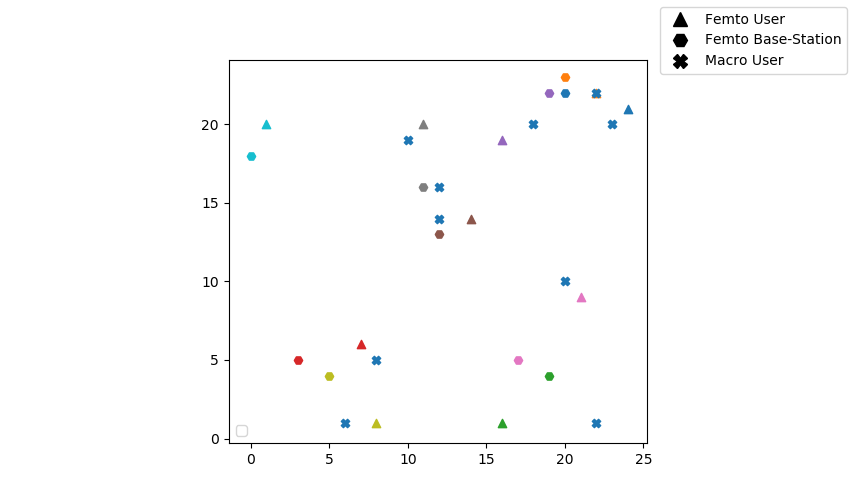
\includegraphics[width=\textwidth,height = 10cm]{figures/system_figure_single}
	  \caption{Simulation Environment: 5 FBSs each with 1 antenna and 1 user in an environment of 10 macro cell users.}
	  \label{system_figure_single}
\end{figure}

\begin{figure}[H]
	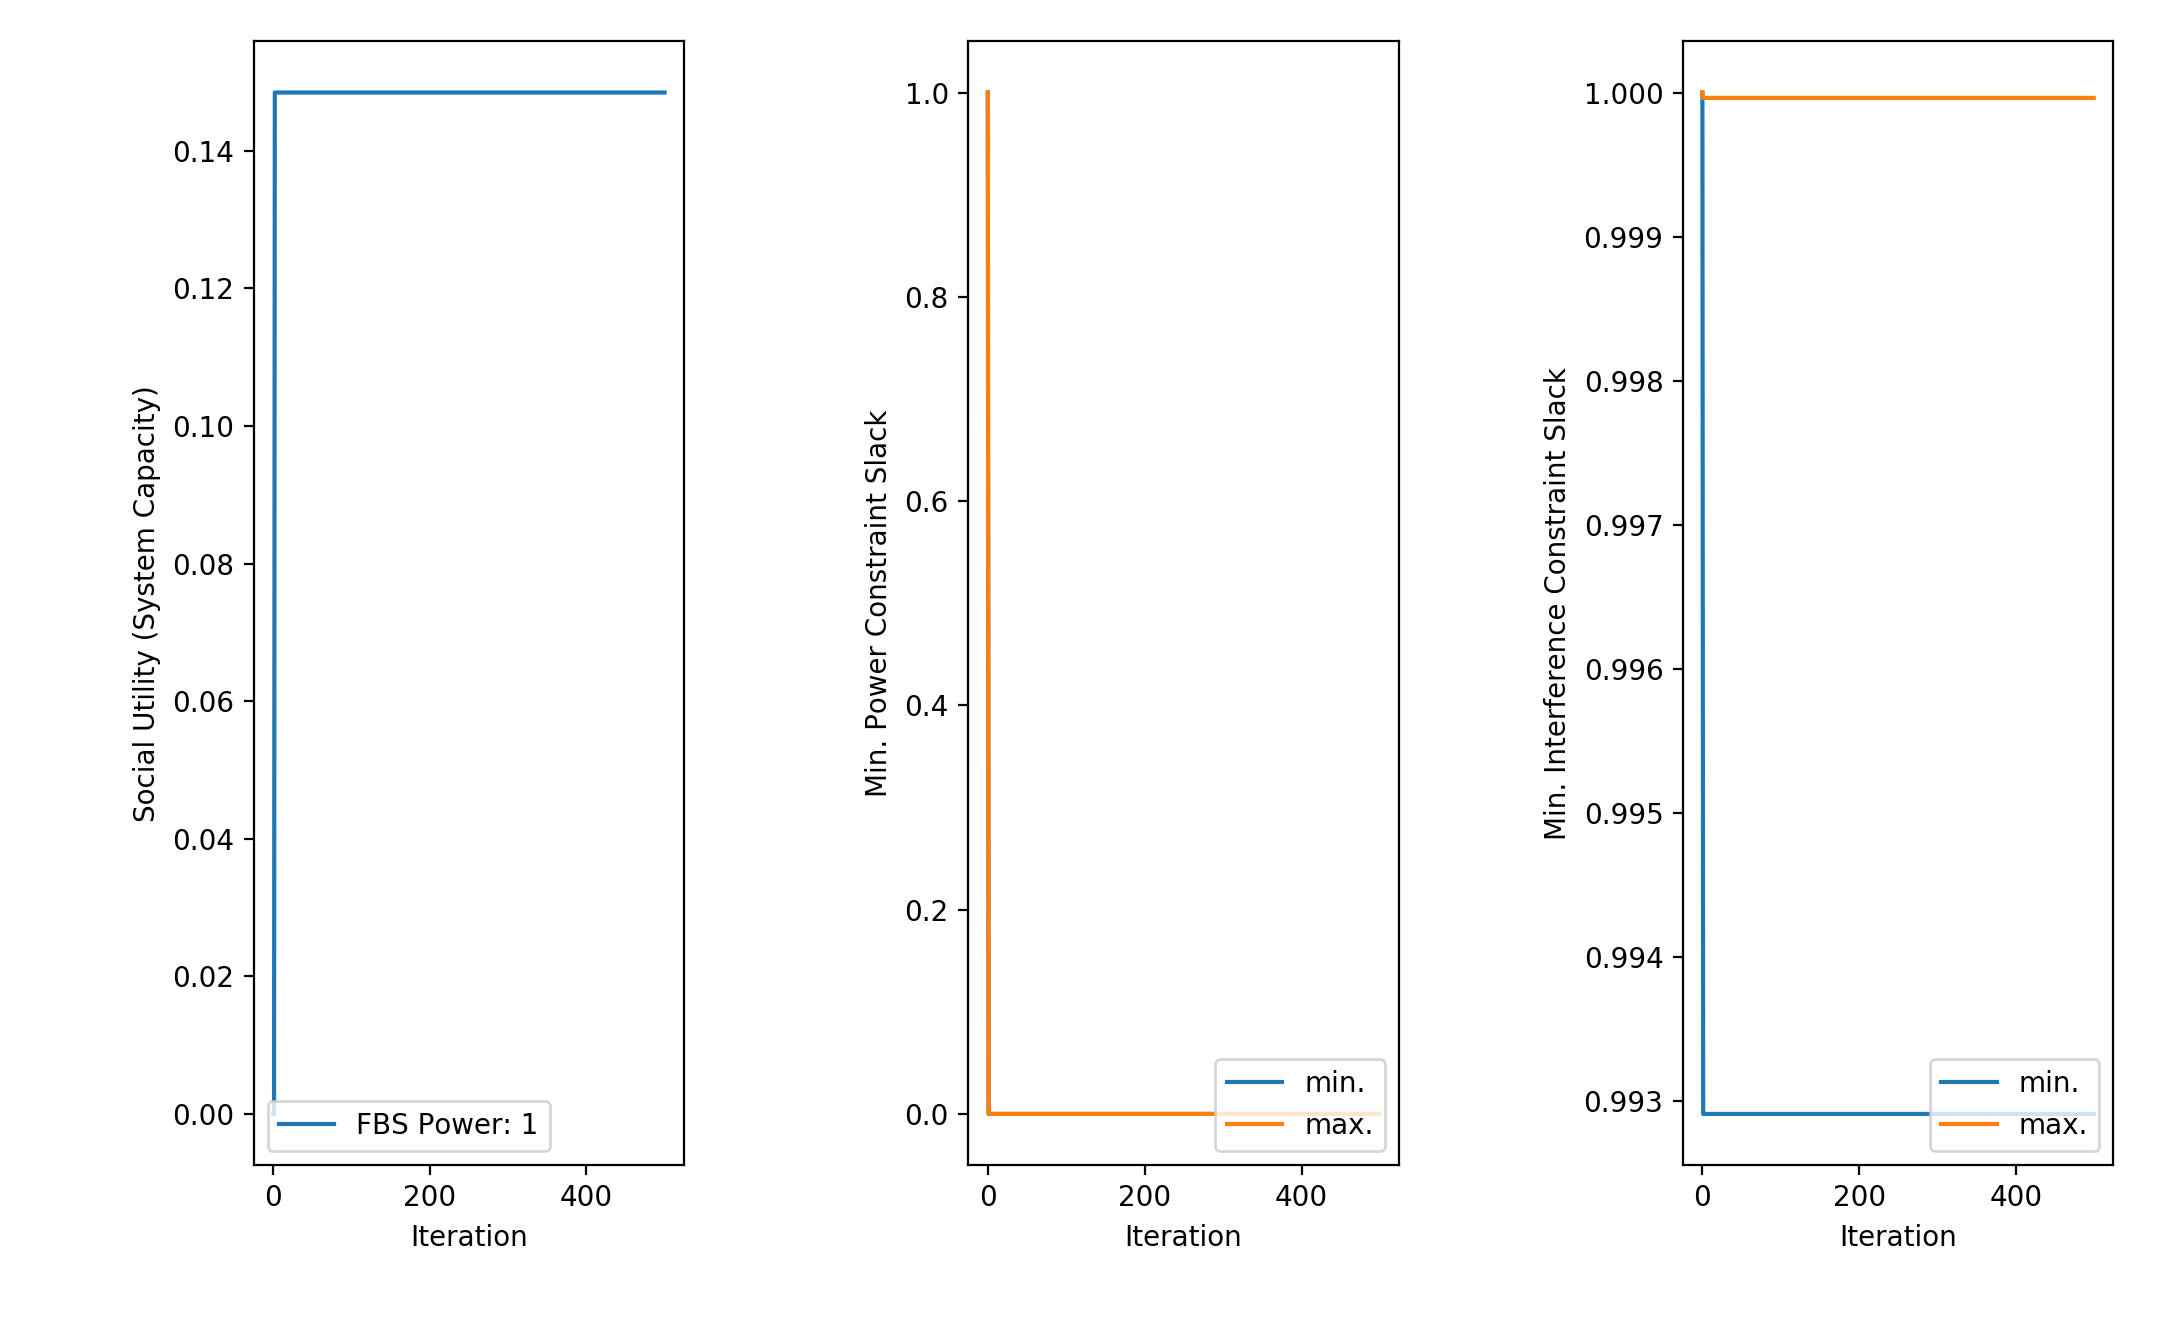
\includegraphics[width= 15cm,height = 10cm]{figures/single_power1}
	  \caption{Single Antenna Game Simulation with total FBS power of 100}
	  \label{single_power1}
\end{figure}
\begin{figure}[H]
	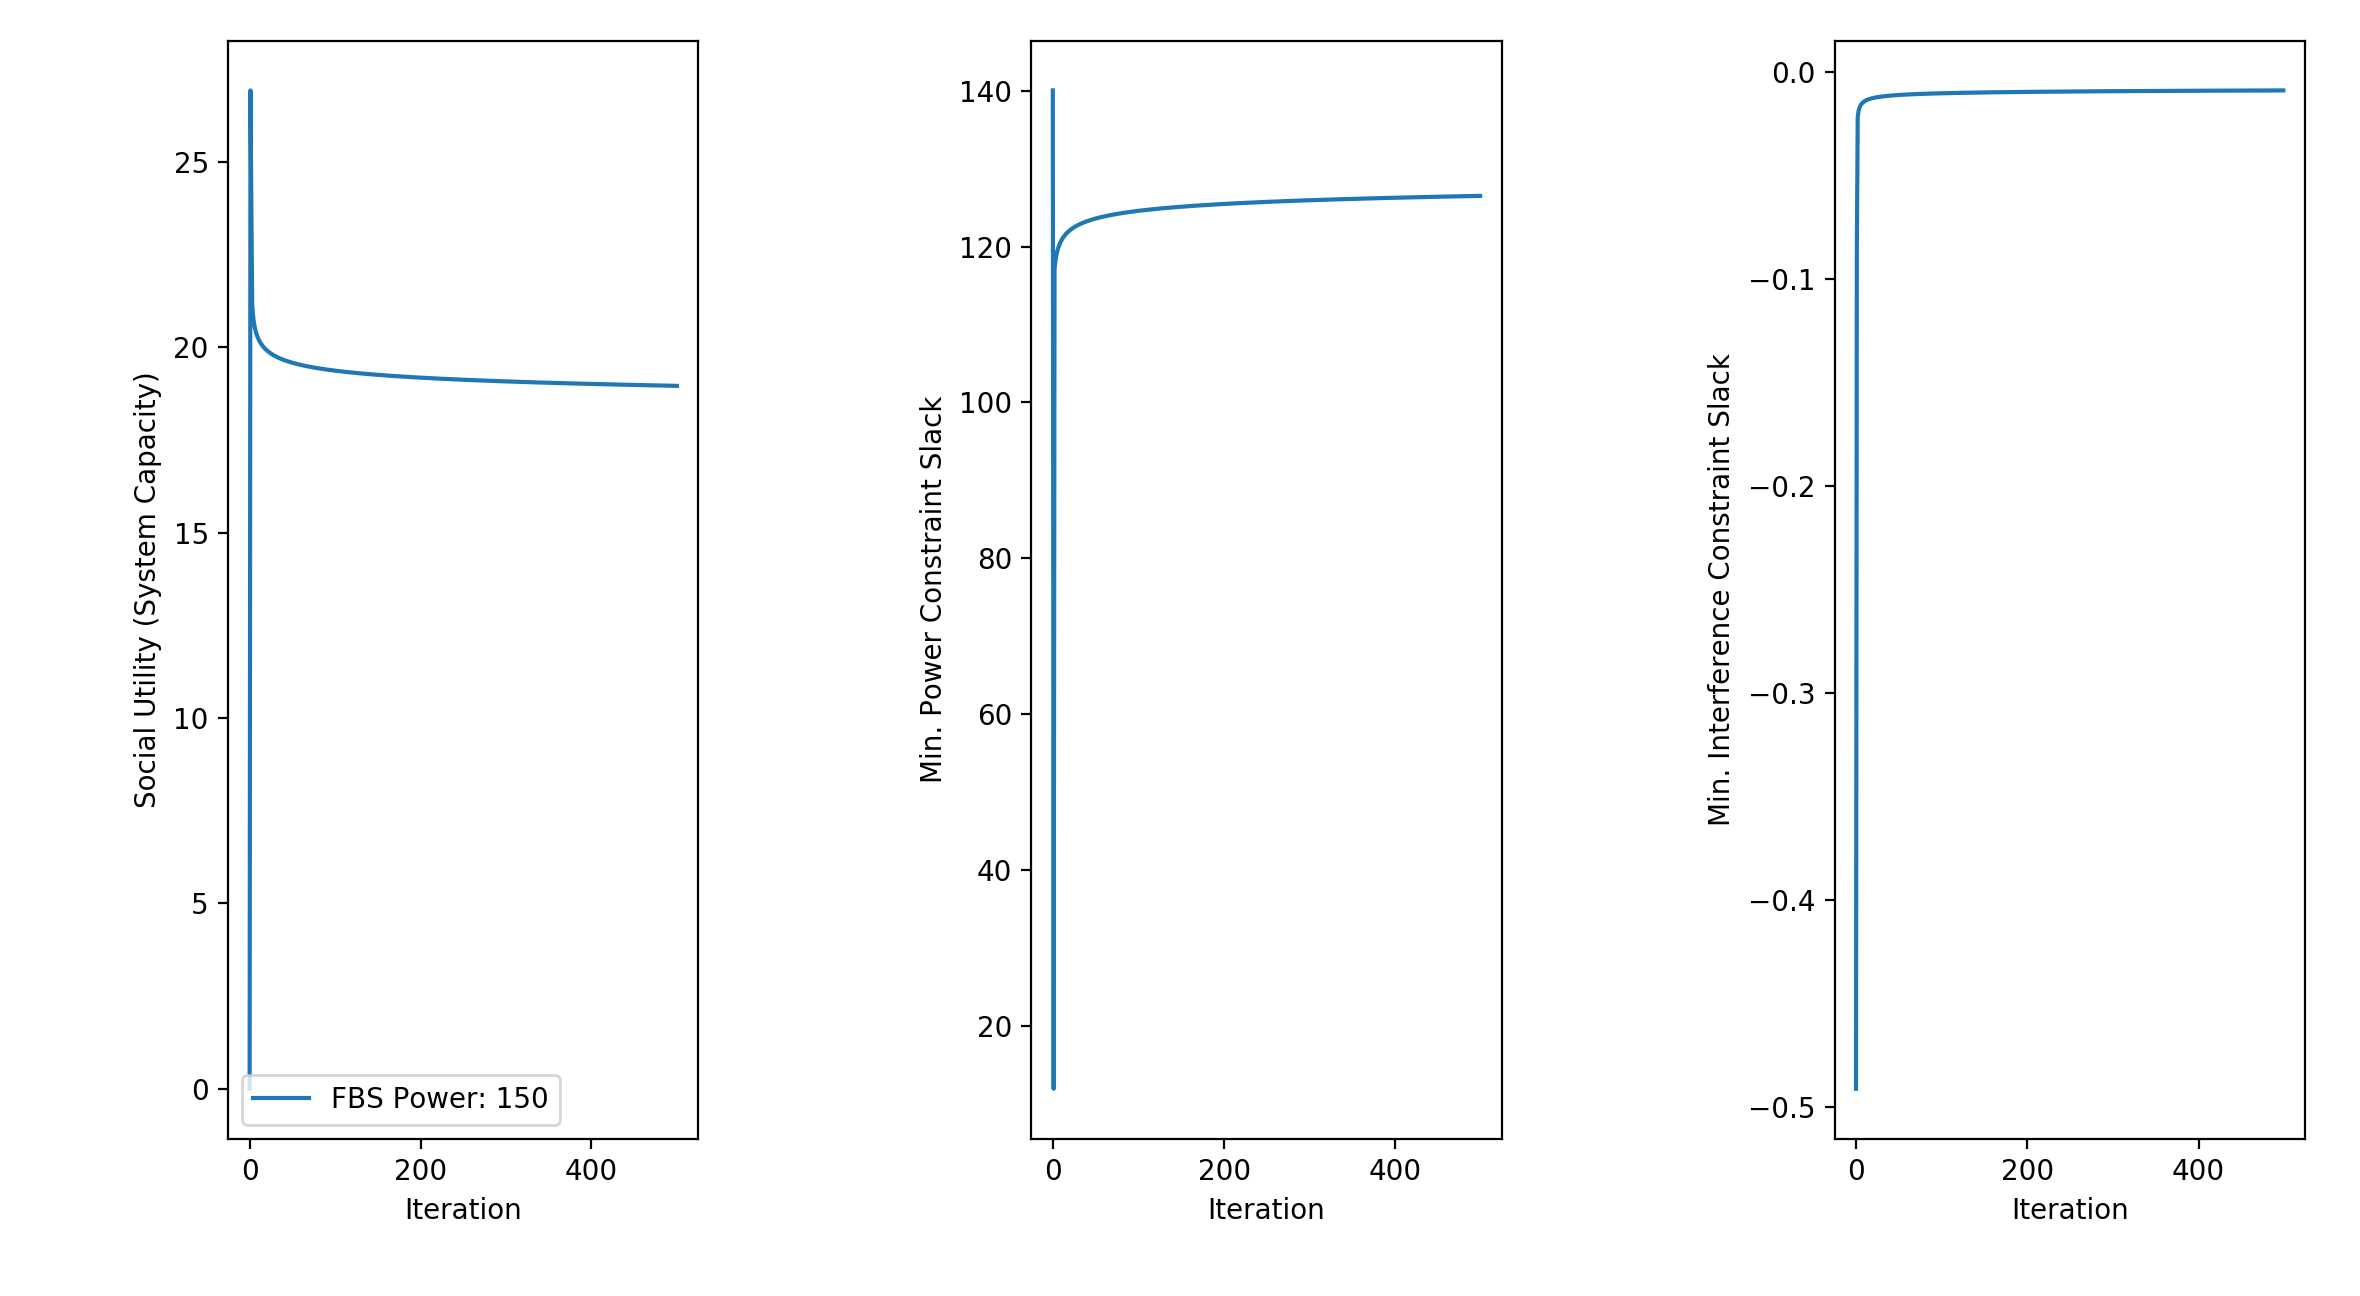
\includegraphics[width= 15cm,height = 10cm]{figures/single_power2}
	  \caption{Single Antenna Game Simulation with total FBS power of 150}
	  \label{single_power2}
\end{figure}


We now consider the case in which FBSs have $T_f > K_f$ such that additional degrees of freedom are available for the choice of beamforming matrix $\mathbf{U}_f$. Figures \ref{multiple_antenna1}, \ref{multiple_antenna2} and \ref{multiple_antenna3} compare the systems with parameters detailed in Table \ref{table2}.
Here we consider the case in which $\mathbf{U}_f$ is chosen according to Problem \ref{mp_opt} to satisfy the zero-forcing constraint (\ref{zf_const_gen}) using the Moore-Penrose inverse. It is seen from Figures \ref{multiple_antenna1}, \ref{multiple_antenna2} and \ref{multiple_antenna3} that when interference is the limiting constraint, additional antennas to the FBS can increase social utility but additional that if too many antennas are available, this method of choosing the beamforming matrix $\mathbf{U}_f$ can lead to decreased utility. This observation further motivates the need for improved methods of choosing $\mathbf{U}_f$.


\begin{center}
\begin{figure}
\begin{tabular}{ | m{8cm} | m{5cm} | } 
\hline
Simulation Area & $30 \times 30$\\ 
\hline
Number of macrocell users & 10\\ 
\hline
Number of FBSs & 5\\ 
\hline
Number of users for each FBSs & 5\\ 
\hline
Number of antennas for each FBSs & 7 (Fig. \ref{multiple_antenna1}), 15 (Fig. \ref{multiple_antenna2}), 30 (Fig. \ref{multiple_antenna3})\\ 
\hline
Noise at femto cell users & $1$\\ 
\hline
FBS power constraint & 1000 \\ 
\hline
Macro user interference threshold & $1$\\ 
\hline
Initial value $p_{f,i}$ & $p_{f,i} = 0$\\
\hline
Initial value of dual variables $\chi_{f}$, $\lambda_{m}$ and $\nu_{f,i}$ & $\nu_{f,i}=1$, $\lambda_{m}=1 $, $\chi_{f}=1$\\
\hline
Dual variable step size $\alpha^k$& $\alpha^k= 1$ $\forall k$\\
\hline
\end{tabular}
\caption{System parameters for Figures \ref{single_power1} and \ref{single_power2}}
\label{table2}
\end{figure}
\end{center}


\begin{figure}[H]
	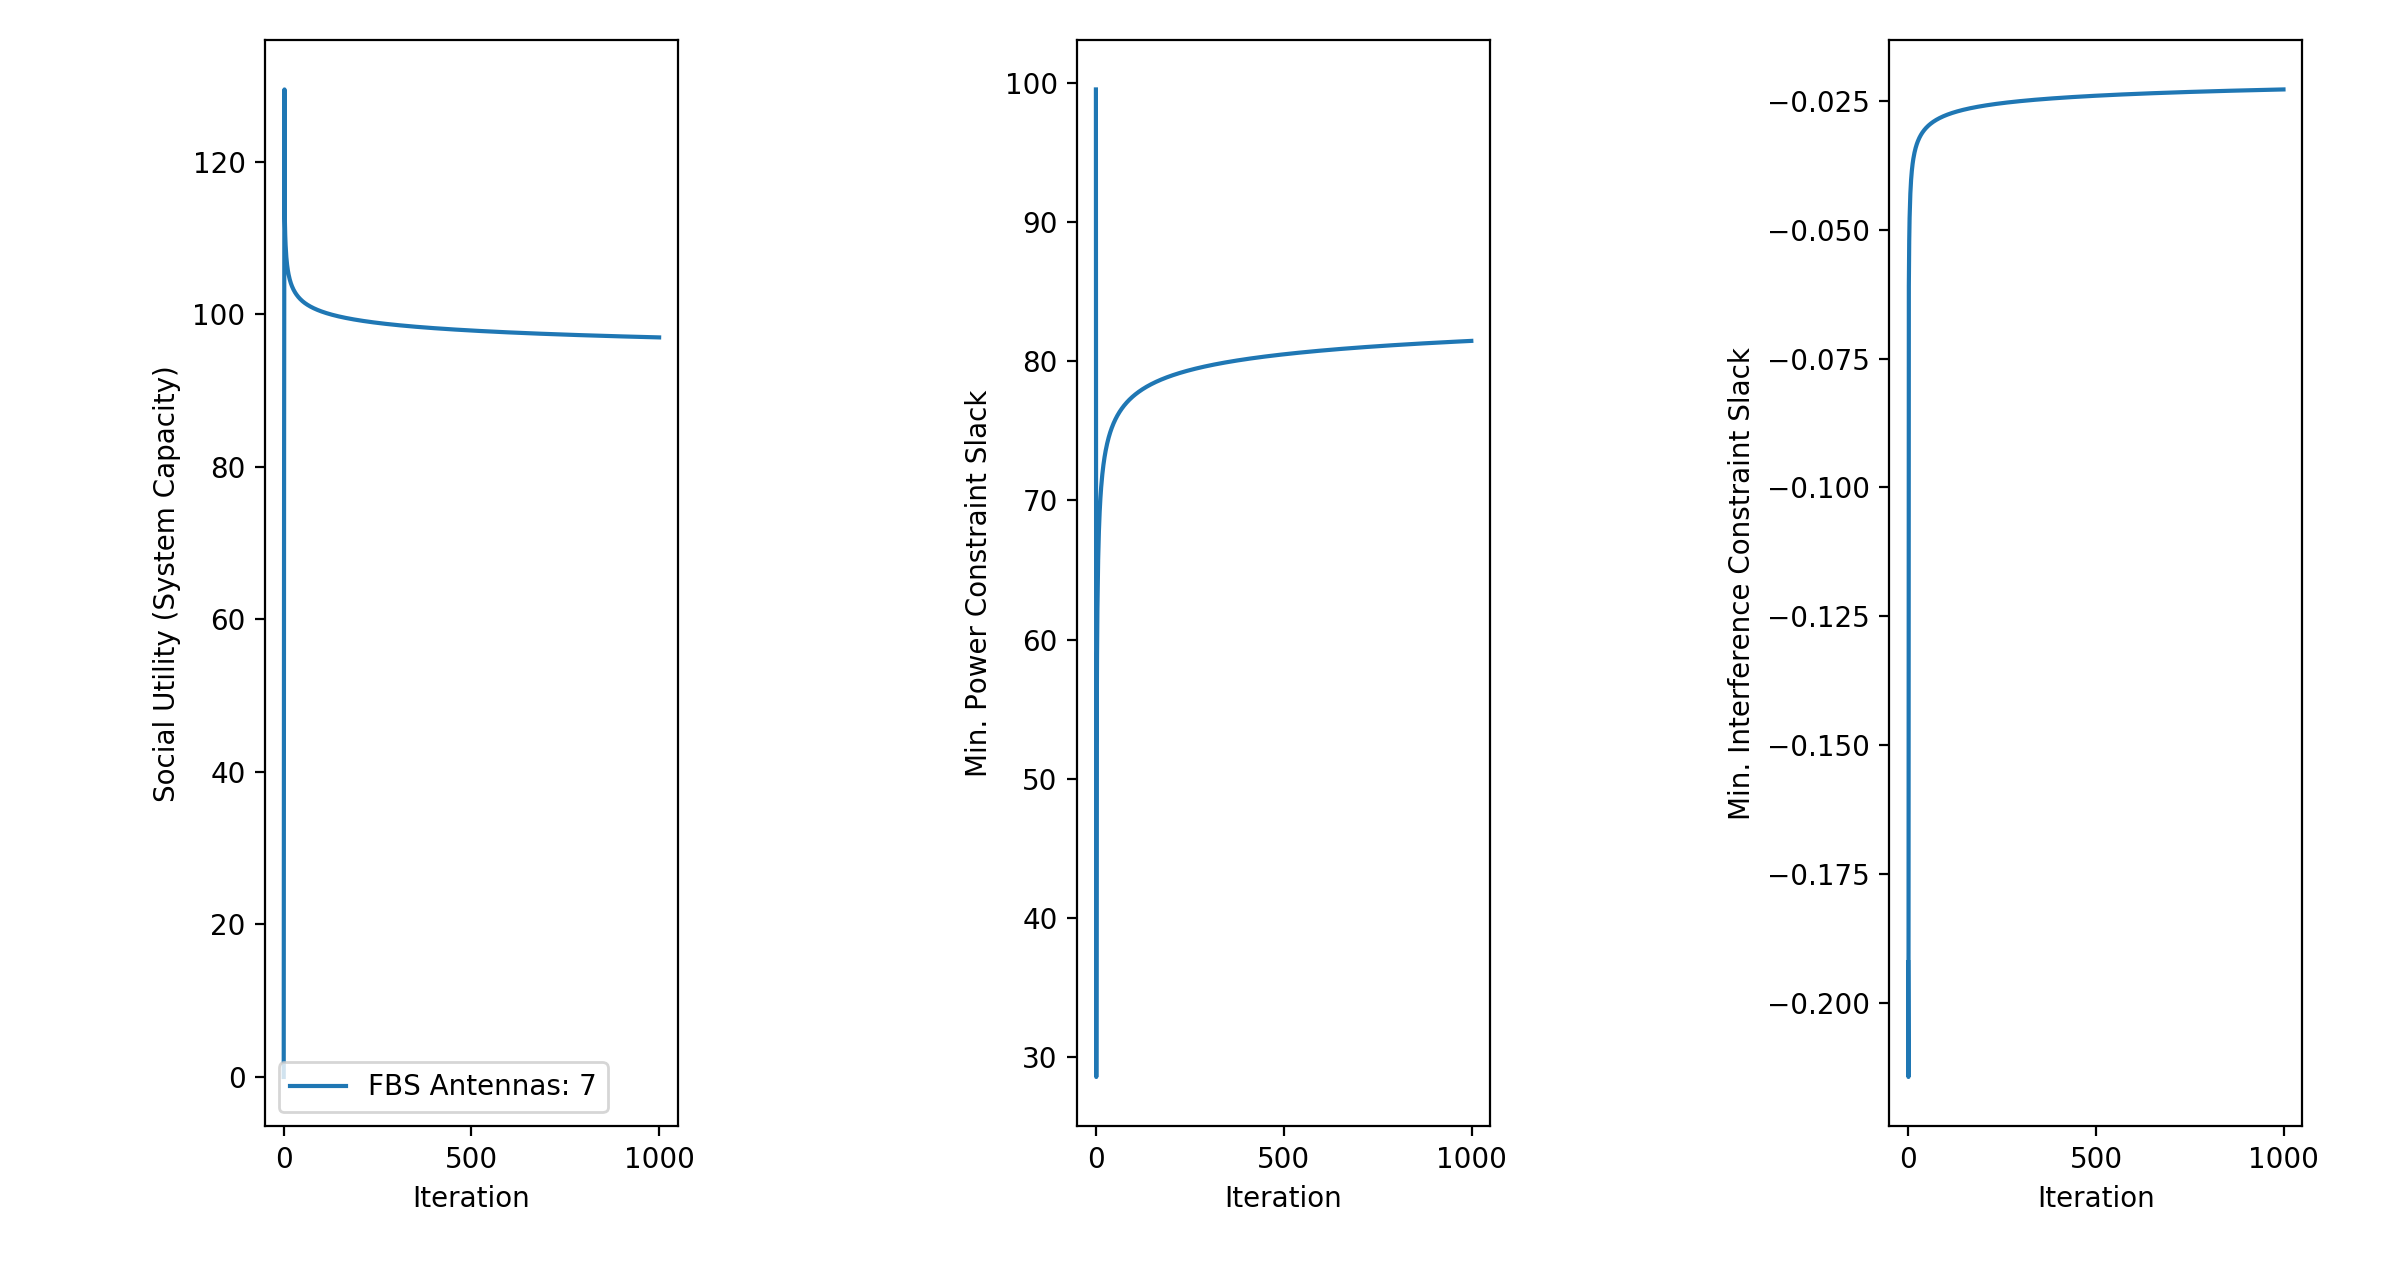
\includegraphics[width= 15cm,height = 10cm]{figures/multiple_antenna1}
	  \caption{Simulation Environment: 5 FBSs each with multiple antennas ($T_f \geq K_f$) and 5 user in an environment of 10 macro cell users.}
	  \label{multiple_antenna1}
\end{figure}

\begin{figure}[H]
	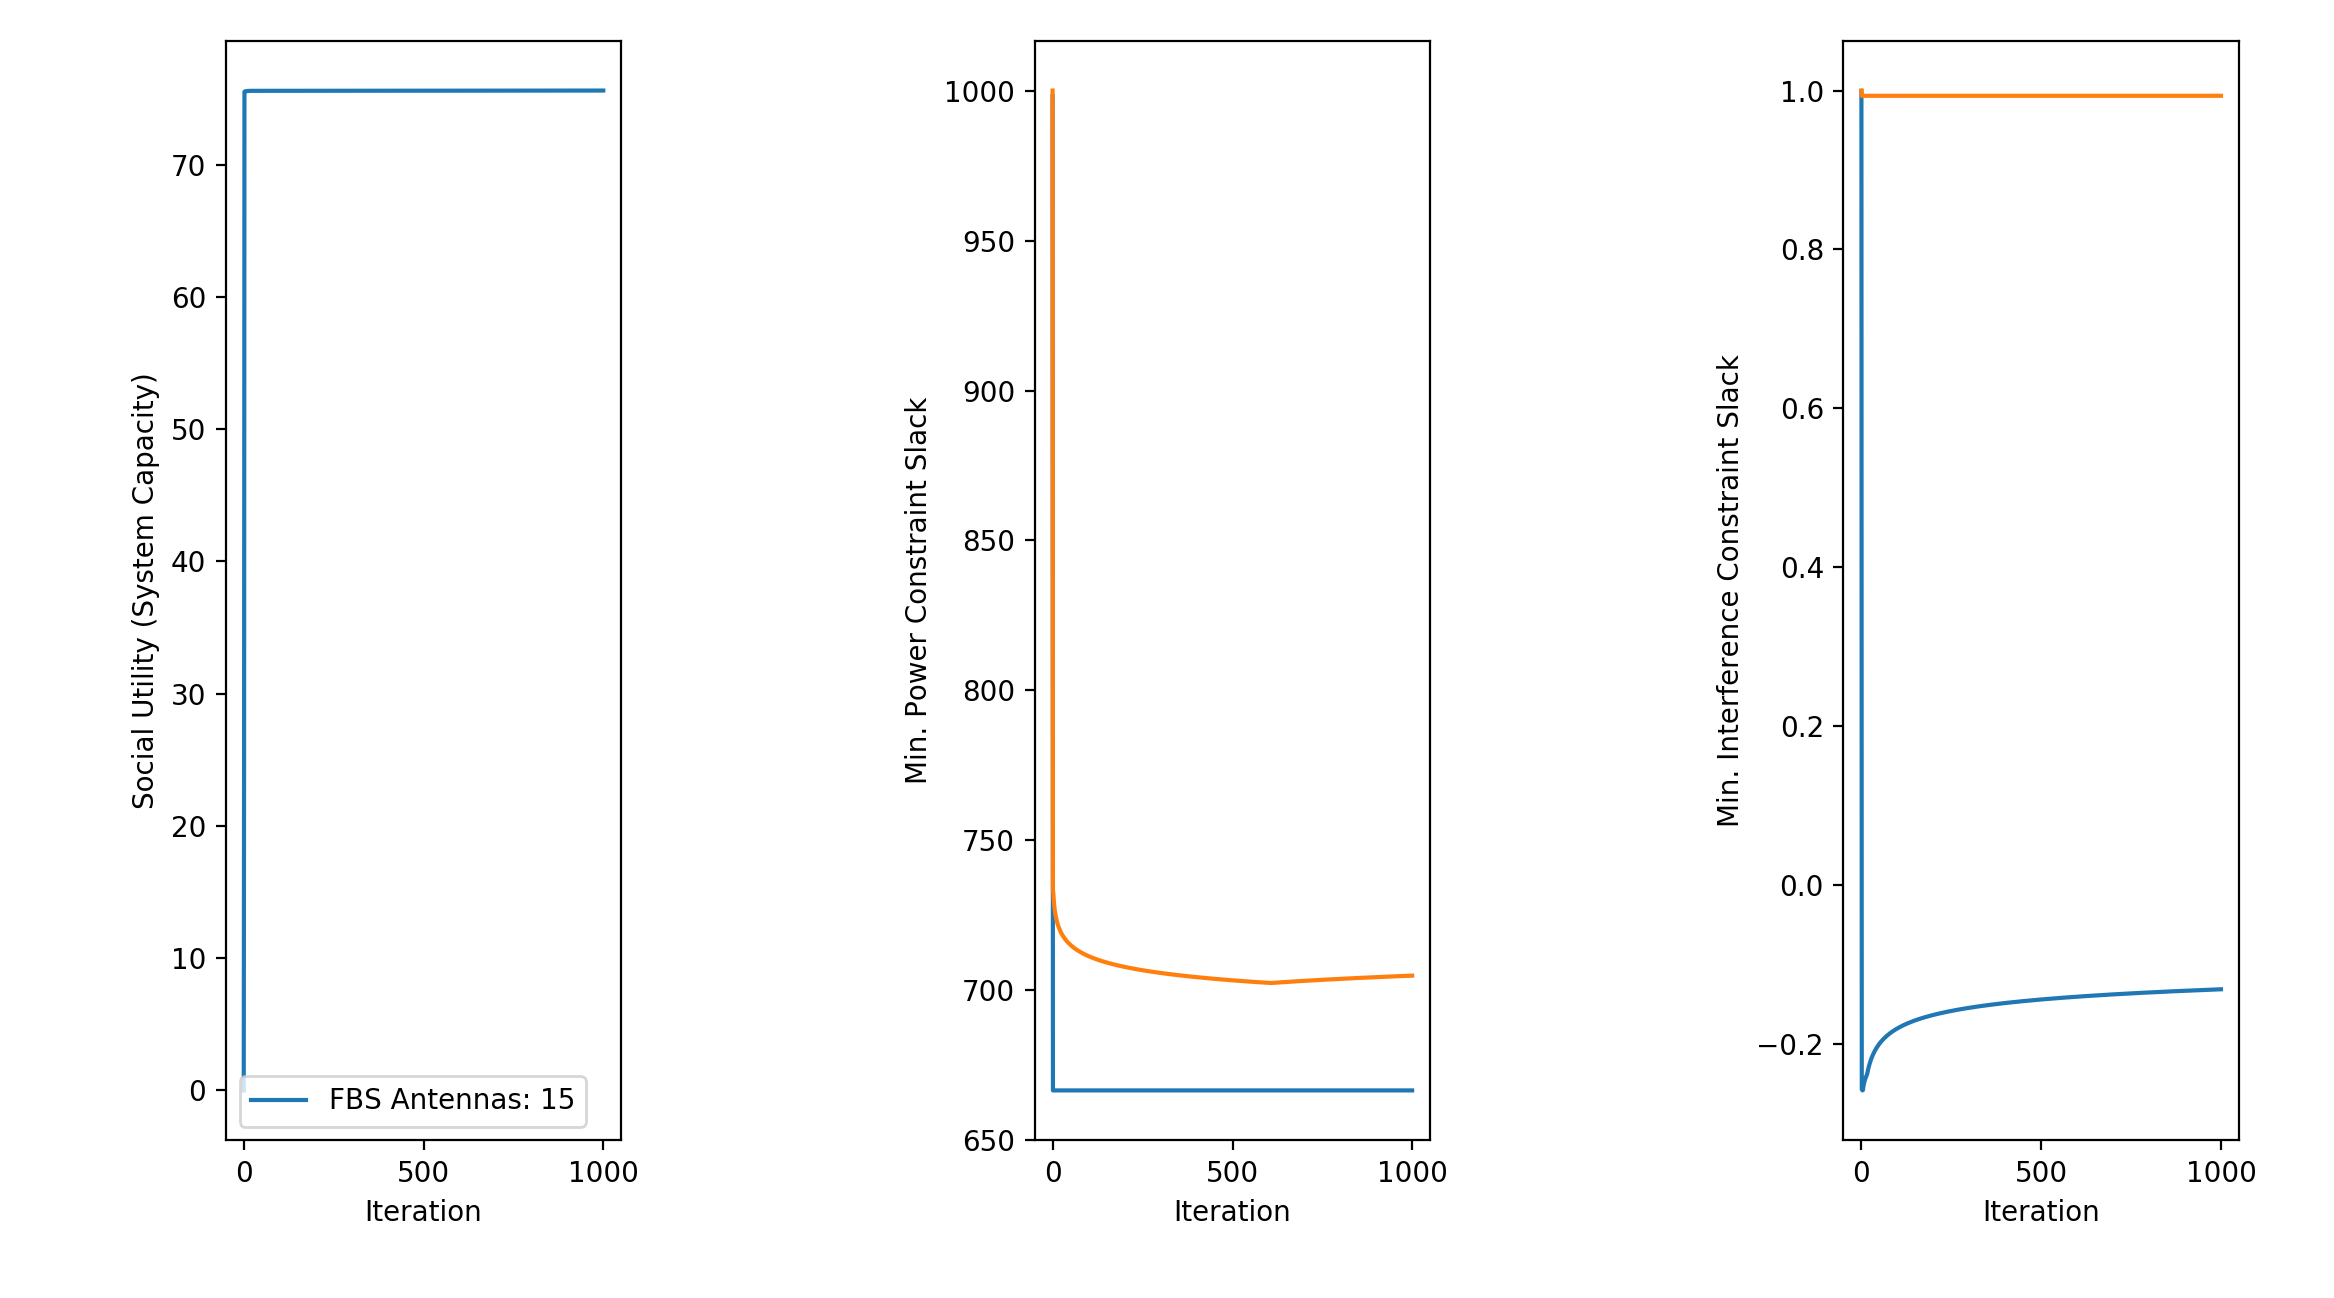
\includegraphics[width=\textwidth,height = 10cm]{figures/multiple_antenna2}
	  \caption{Multiple antenna simulation for FBSs with 15 antennas and 5 users.
	  }
	  \label{multiple_antenna2}
\end{figure}

\begin{figure}[H]
	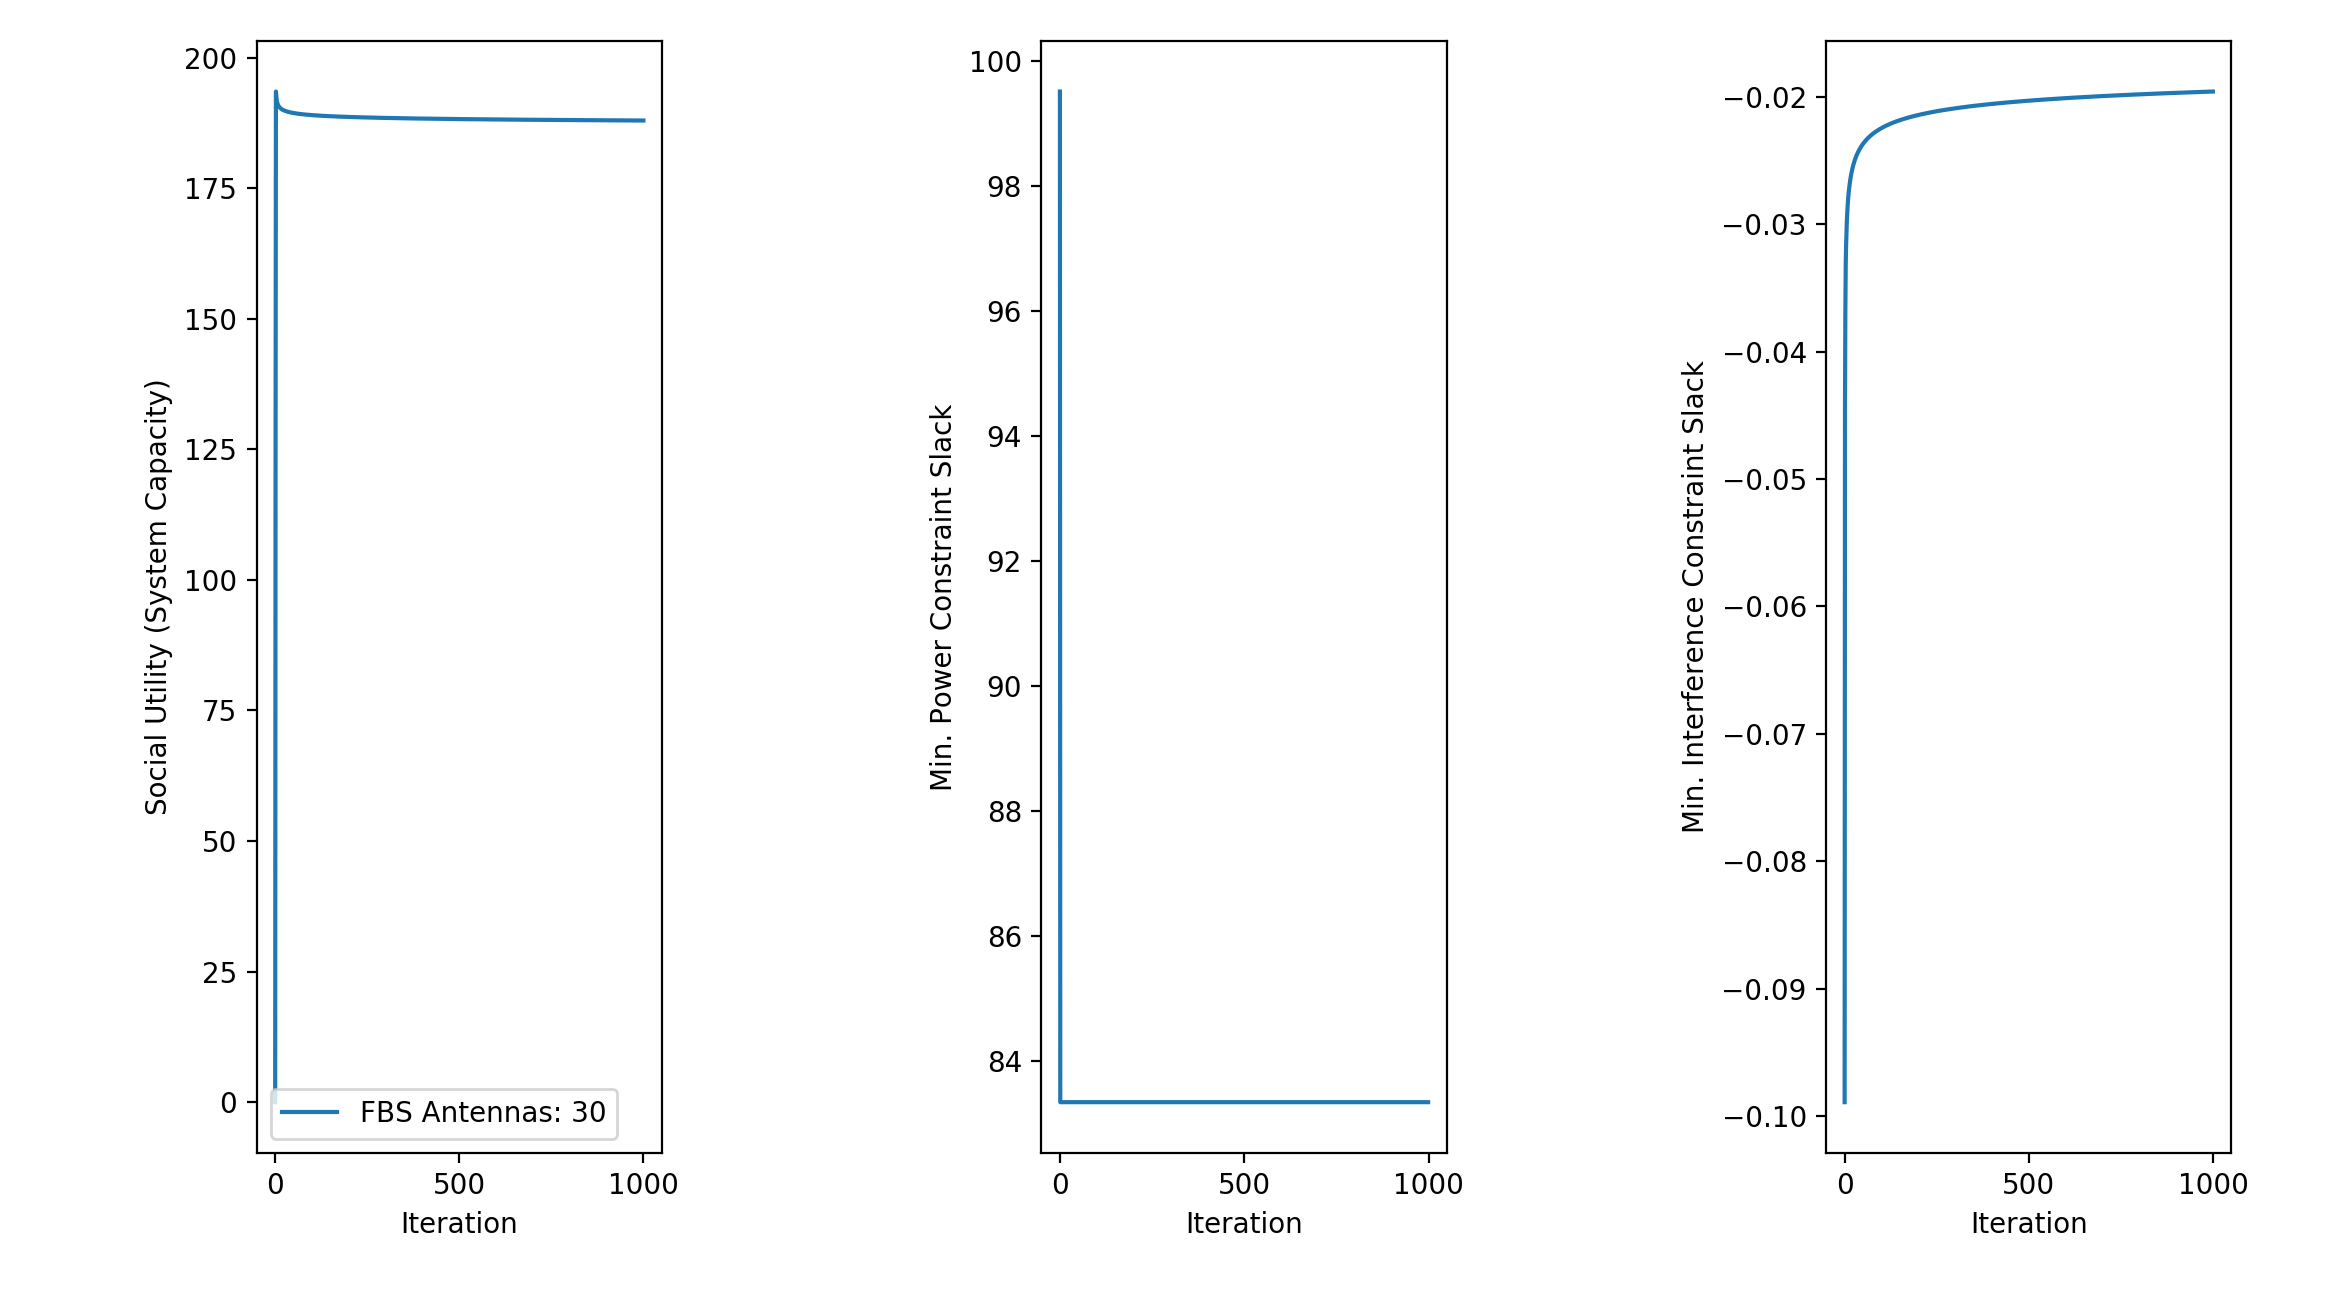
\includegraphics[width=\textwidth,height = 10cm]{figures/multiple_antenna3}
	  \caption{Multiple antenna simulation for FBSs with 30 antennas and 5 users.
	  }
	  \label{multiple_antenna3}
\end{figure}


Last, using the simulation parameters from Table \ref{table2}, we compare the game when $\mathbf{U}_f$ is chosen according to the solutions of Problems \ref{mp_opt}, and \ref{correlation_opt}. The results in Figures \ref{beamformer_comparison} and \ref{beamformer_comparison2} are generated by placing the user and base station locations randomly. These two example are presented to illustrate the following two scenarios. First, in the case (Fig. \ref{beamformer_comparison}) that macro user channels are highly correlated to the user channels of FBSs, we see that Moore-Penrose beamformer resulting from Problem \ref{mp_opt} outperforms the beamformer from Problem \ref{correlation_opt}, minimizing correlation with macro users. In contrast, we see that when user channels are \emph{not} correlated with macro user channels (Fig. \ref{beamformer_comparison2}), the correlation minimizing beamformer can outperform the Moore-Penrose beamformer by utilizing the full power available at the FBS.  

\begin{figure}[H]
	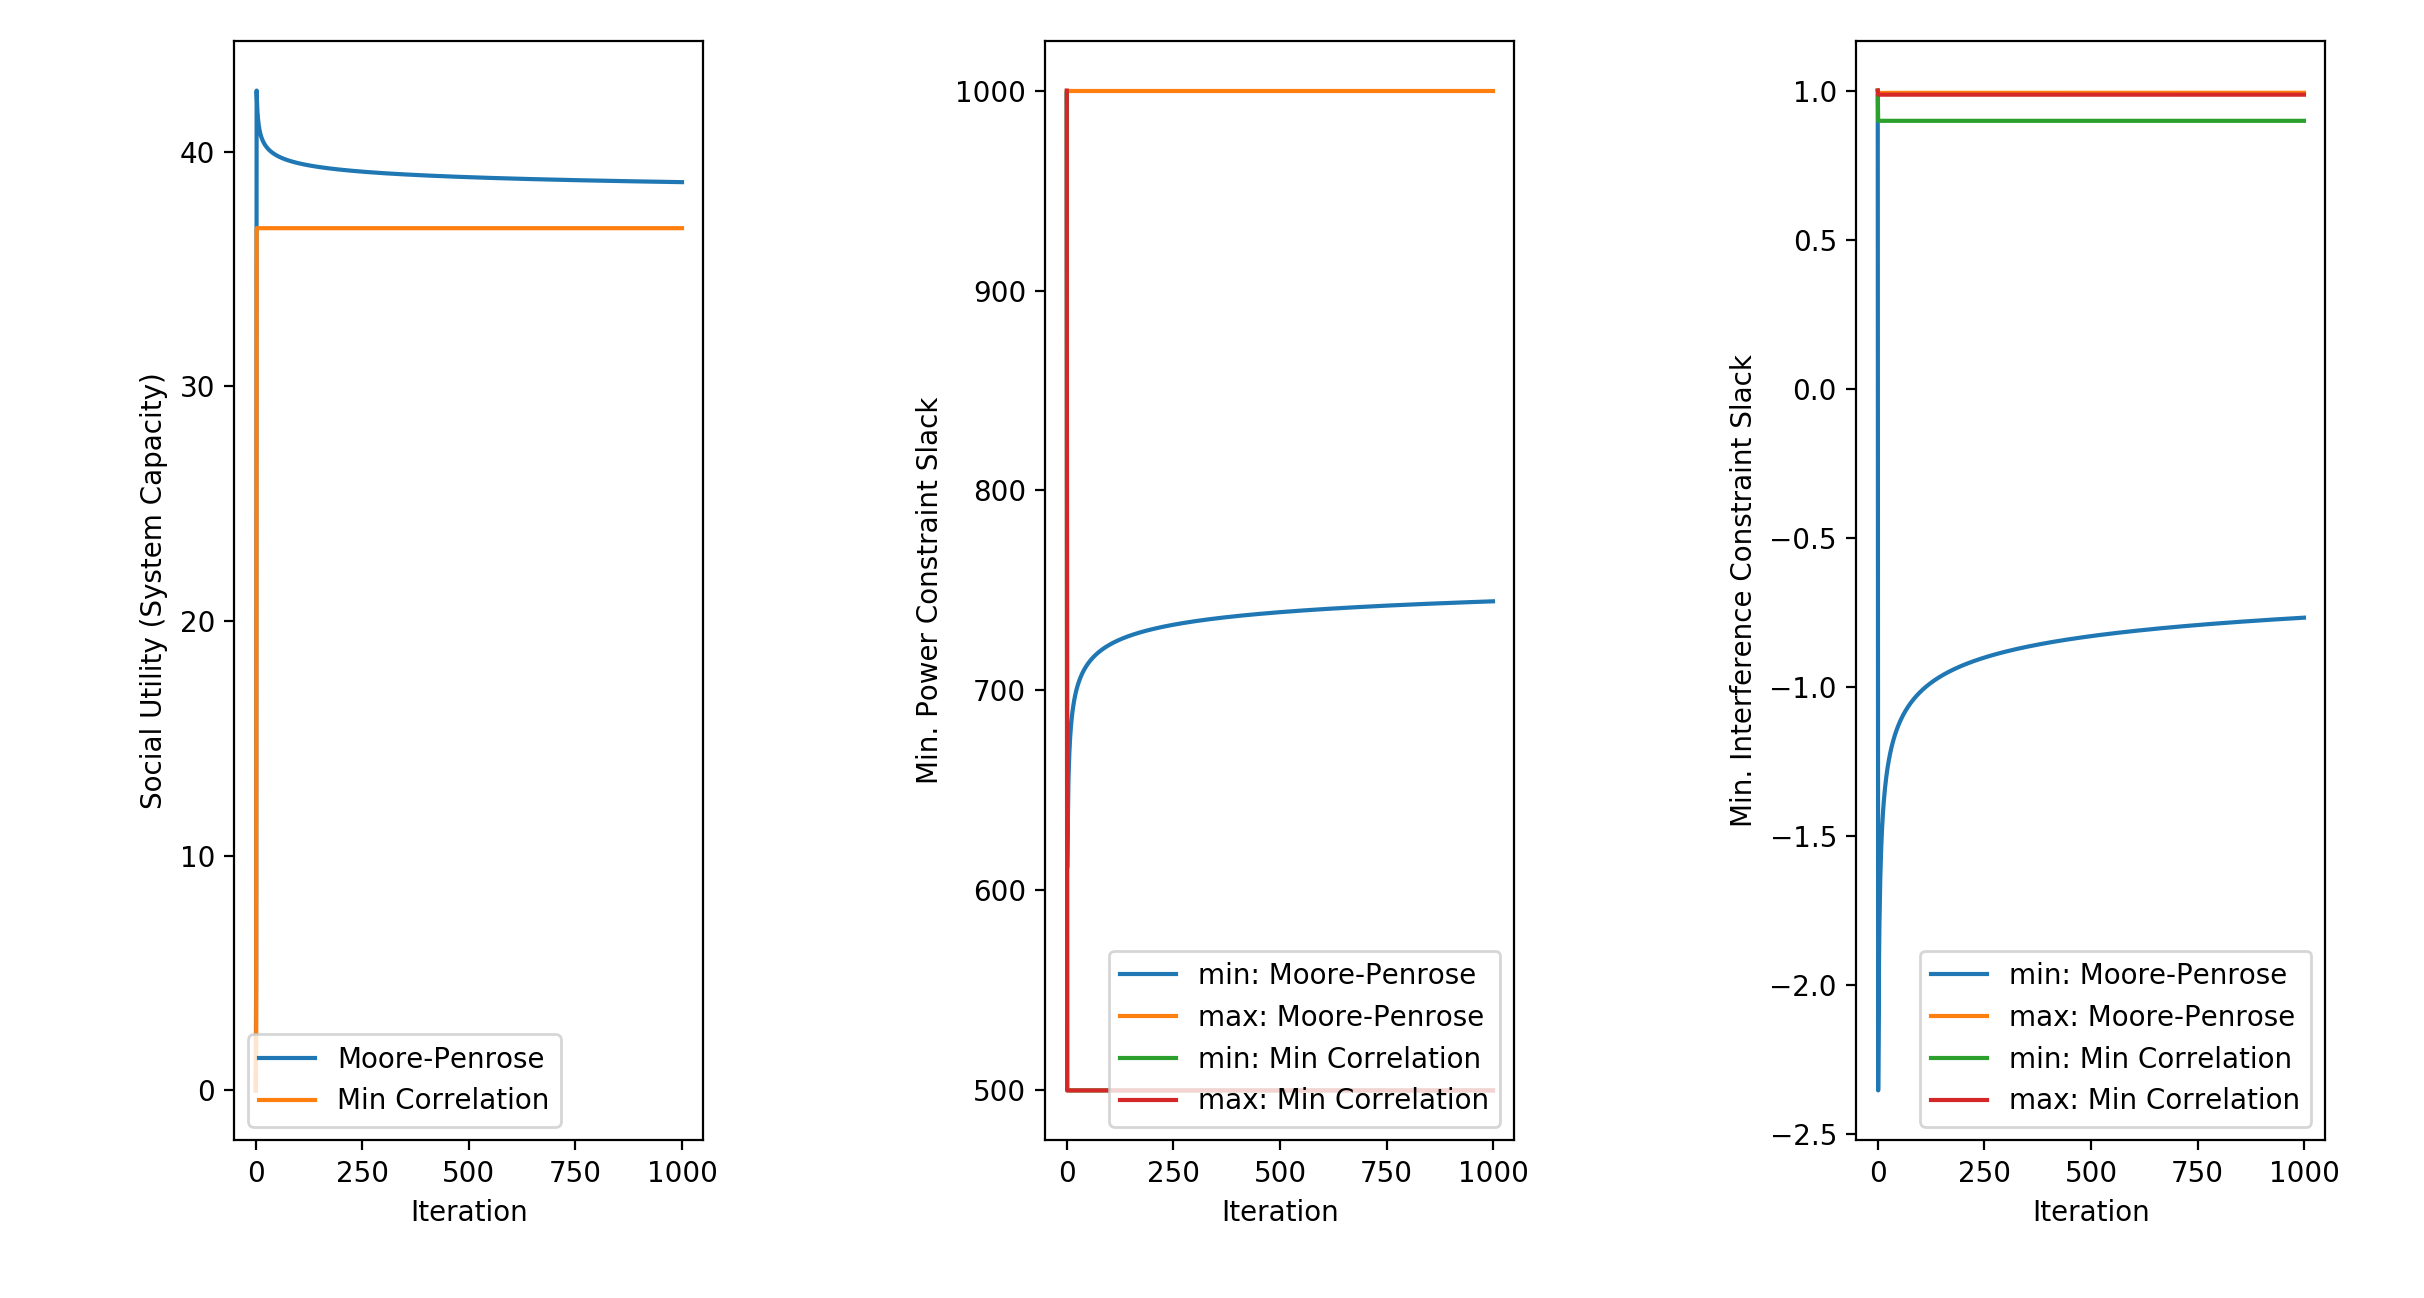
\includegraphics[width= 15cm,height = 10cm]{figures/beamformer_comparison}
	  \caption{First comparison scenario between choices for beamformer $\mathbf{U}_f$ using the solutions to the optimization problems in \ref{mp_opt}, and \ref{correlation_opt}.}
	  \label{beamformer_comparison}
\end{figure}

\begin{figure}[H]
	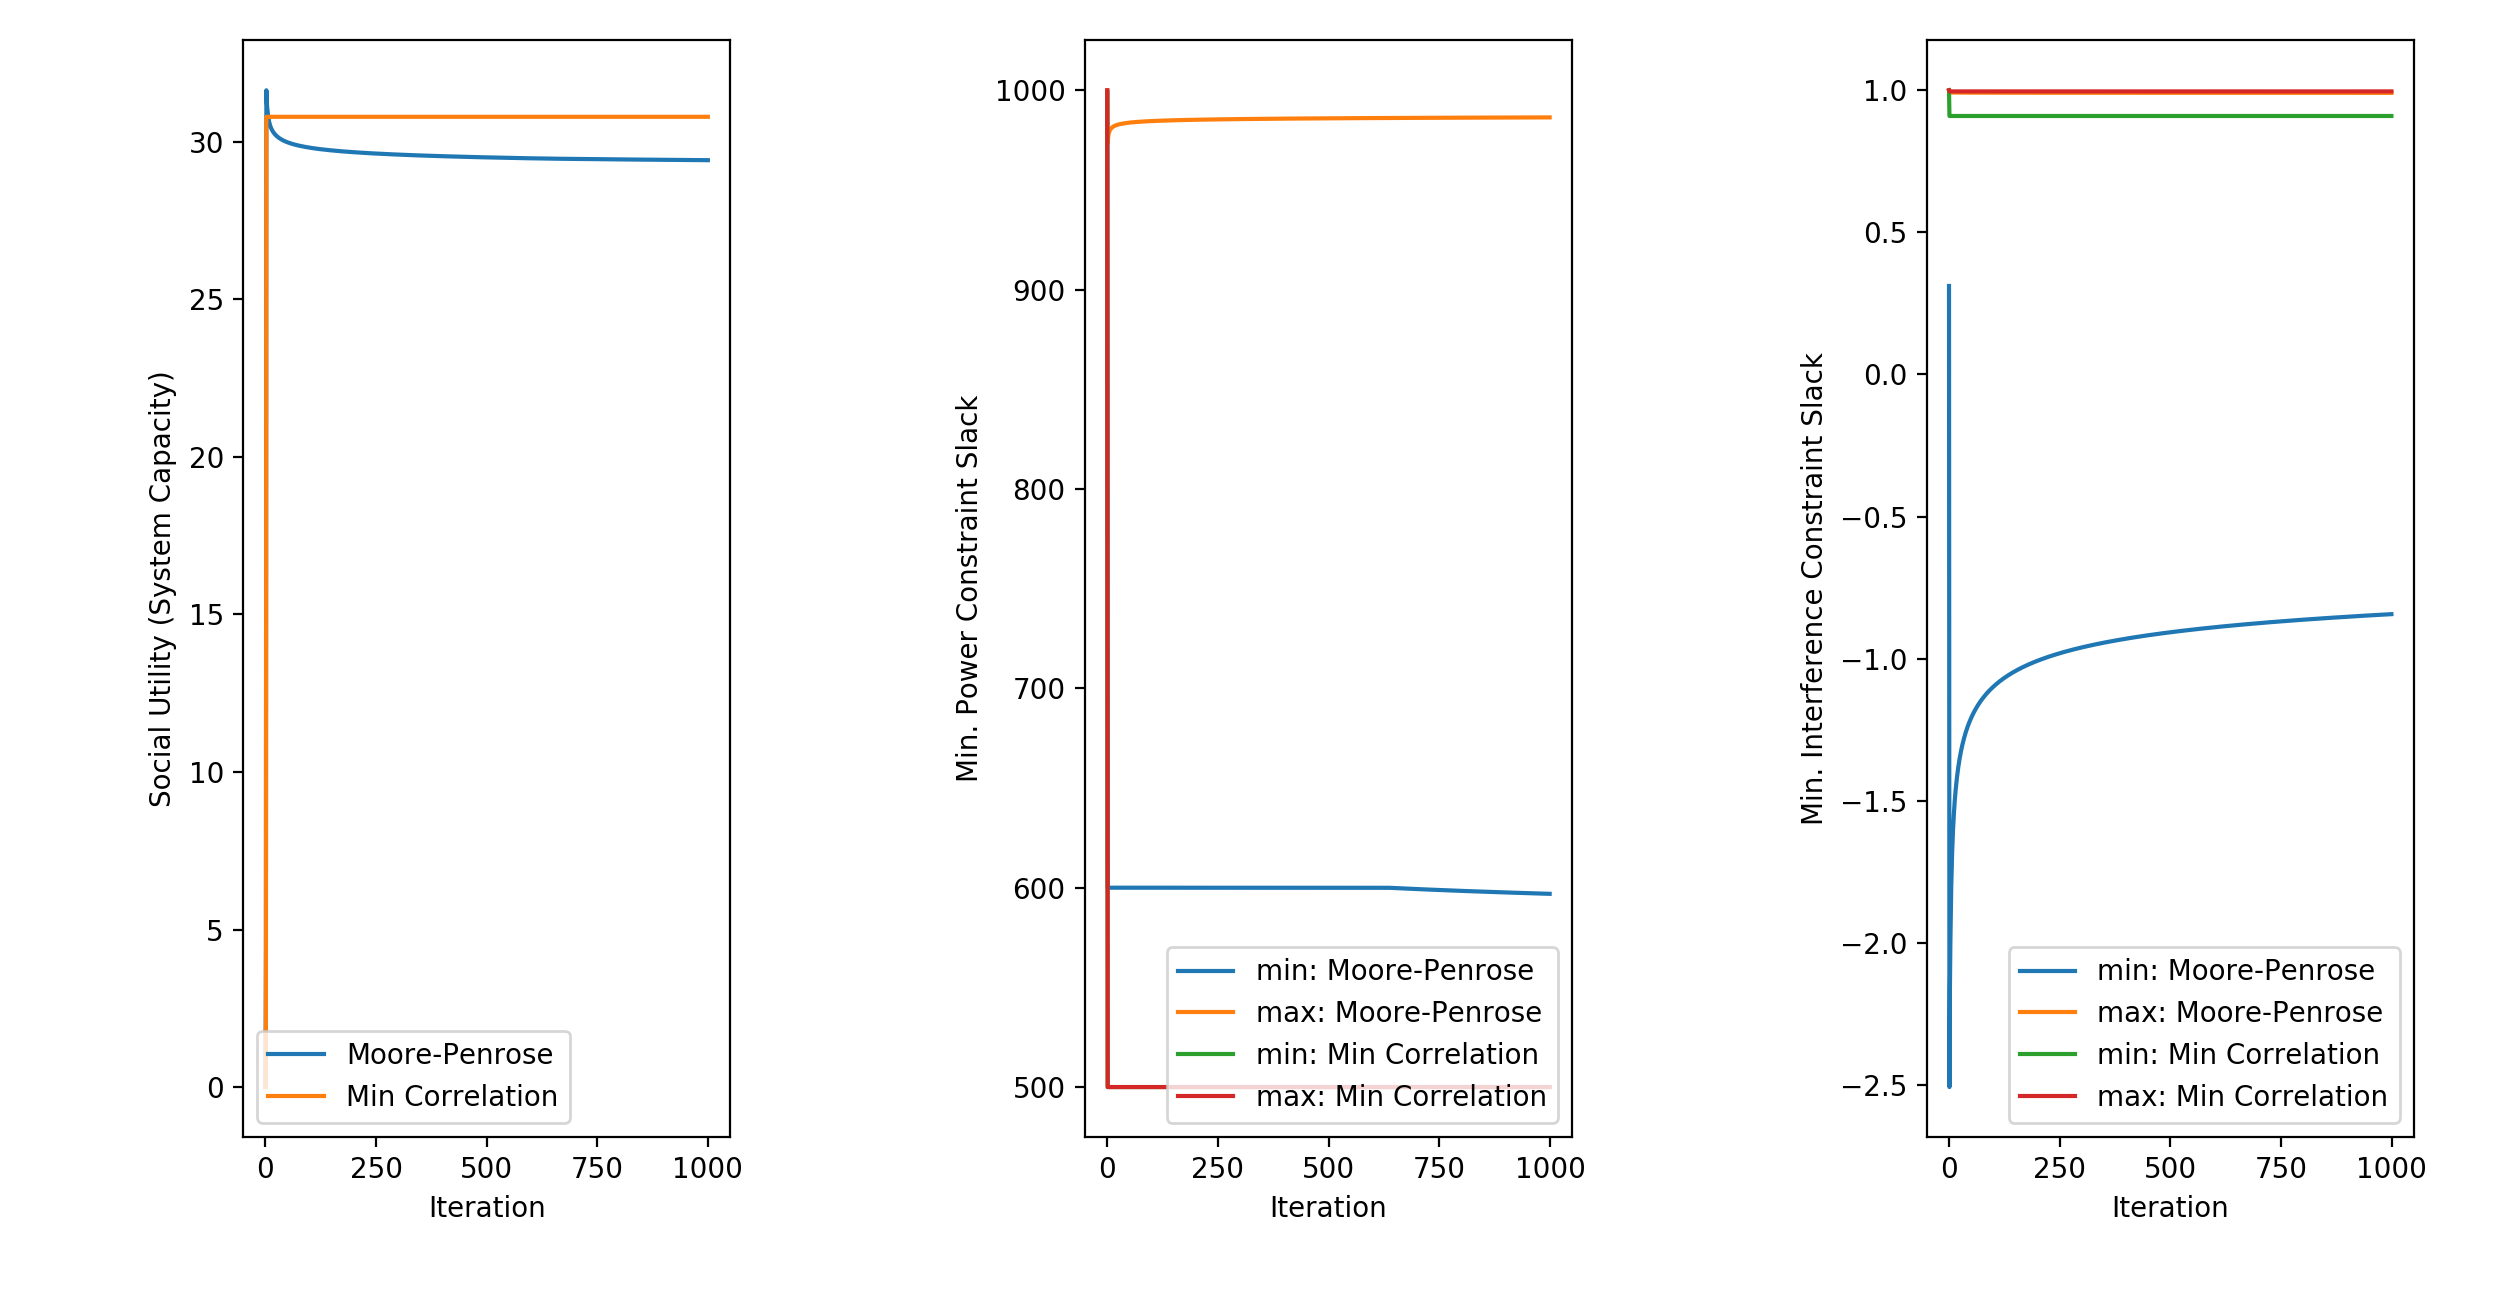
\includegraphics[width= 15cm,height = 10cm]{figures/beamformer_comparison2}
	  \caption{Second comparison scenario between choices for beamformer $\mathbf{U}_f$ using the solutions to the optimization problems in \ref{mp_opt}, and \ref{correlation_opt}.}
	  \label{beamformer_comparison2}
\end{figure}


\chapter{Conclusion}
In this work, the power allocation problem for heterogeneous networks with femto cell base stations has been analyzed. The most general setup of this problem poses difficulties for distributed solutions due to the non-concavity of the resulting utility functions. It is shown that under additional beam-forming constraints on base stations equipped with antenna arrays, a unique, normalized Nash equilibrium can be achieved with a distributed solution. 
\par
Future work should extend the system presented here to further generalizations including interference between the femtocell basestations, and potential games for imperfect channel estimation. 